\documentclass[]{article}
\usepackage{lmodern}
\usepackage{amssymb,amsmath}
\usepackage{ifxetex,ifluatex}
\usepackage{fixltx2e} % provides \textsubscript
\ifnum 0\ifxetex 1\fi\ifluatex 1\fi=0 % if pdftex
  \usepackage[T1]{fontenc}
  \usepackage[utf8]{inputenc}
\else % if luatex or xelatex
  \ifxetex
    \usepackage{mathspec}
  \else
    \usepackage{fontspec}
  \fi
  \defaultfontfeatures{Ligatures=TeX,Scale=MatchLowercase}
\fi
% use upquote if available, for straight quotes in verbatim environments
\IfFileExists{upquote.sty}{\usepackage{upquote}}{}
% use microtype if available
\IfFileExists{microtype.sty}{%
\usepackage{microtype}
\UseMicrotypeSet[protrusion]{basicmath} % disable protrusion for tt fonts
}{}
\usepackage[margin=1in]{geometry}
\usepackage{hyperref}
\hypersetup{unicode=true,
            pdftitle={Homework\_1},
            pdfauthor={Zhoumengdi Wang (zxw534)},
            pdfborder={0 0 0},
            breaklinks=true}
\urlstyle{same}  % don't use monospace font for urls
\usepackage{color}
\usepackage{fancyvrb}
\newcommand{\VerbBar}{|}
\newcommand{\VERB}{\Verb[commandchars=\\\{\}]}
\DefineVerbatimEnvironment{Highlighting}{Verbatim}{commandchars=\\\{\}}
% Add ',fontsize=\small' for more characters per line
\usepackage{framed}
\definecolor{shadecolor}{RGB}{248,248,248}
\newenvironment{Shaded}{\begin{snugshade}}{\end{snugshade}}
\newcommand{\KeywordTok}[1]{\textcolor[rgb]{0.13,0.29,0.53}{\textbf{#1}}}
\newcommand{\DataTypeTok}[1]{\textcolor[rgb]{0.13,0.29,0.53}{#1}}
\newcommand{\DecValTok}[1]{\textcolor[rgb]{0.00,0.00,0.81}{#1}}
\newcommand{\BaseNTok}[1]{\textcolor[rgb]{0.00,0.00,0.81}{#1}}
\newcommand{\FloatTok}[1]{\textcolor[rgb]{0.00,0.00,0.81}{#1}}
\newcommand{\ConstantTok}[1]{\textcolor[rgb]{0.00,0.00,0.00}{#1}}
\newcommand{\CharTok}[1]{\textcolor[rgb]{0.31,0.60,0.02}{#1}}
\newcommand{\SpecialCharTok}[1]{\textcolor[rgb]{0.00,0.00,0.00}{#1}}
\newcommand{\StringTok}[1]{\textcolor[rgb]{0.31,0.60,0.02}{#1}}
\newcommand{\VerbatimStringTok}[1]{\textcolor[rgb]{0.31,0.60,0.02}{#1}}
\newcommand{\SpecialStringTok}[1]{\textcolor[rgb]{0.31,0.60,0.02}{#1}}
\newcommand{\ImportTok}[1]{#1}
\newcommand{\CommentTok}[1]{\textcolor[rgb]{0.56,0.35,0.01}{\textit{#1}}}
\newcommand{\DocumentationTok}[1]{\textcolor[rgb]{0.56,0.35,0.01}{\textbf{\textit{#1}}}}
\newcommand{\AnnotationTok}[1]{\textcolor[rgb]{0.56,0.35,0.01}{\textbf{\textit{#1}}}}
\newcommand{\CommentVarTok}[1]{\textcolor[rgb]{0.56,0.35,0.01}{\textbf{\textit{#1}}}}
\newcommand{\OtherTok}[1]{\textcolor[rgb]{0.56,0.35,0.01}{#1}}
\newcommand{\FunctionTok}[1]{\textcolor[rgb]{0.00,0.00,0.00}{#1}}
\newcommand{\VariableTok}[1]{\textcolor[rgb]{0.00,0.00,0.00}{#1}}
\newcommand{\ControlFlowTok}[1]{\textcolor[rgb]{0.13,0.29,0.53}{\textbf{#1}}}
\newcommand{\OperatorTok}[1]{\textcolor[rgb]{0.81,0.36,0.00}{\textbf{#1}}}
\newcommand{\BuiltInTok}[1]{#1}
\newcommand{\ExtensionTok}[1]{#1}
\newcommand{\PreprocessorTok}[1]{\textcolor[rgb]{0.56,0.35,0.01}{\textit{#1}}}
\newcommand{\AttributeTok}[1]{\textcolor[rgb]{0.77,0.63,0.00}{#1}}
\newcommand{\RegionMarkerTok}[1]{#1}
\newcommand{\InformationTok}[1]{\textcolor[rgb]{0.56,0.35,0.01}{\textbf{\textit{#1}}}}
\newcommand{\WarningTok}[1]{\textcolor[rgb]{0.56,0.35,0.01}{\textbf{\textit{#1}}}}
\newcommand{\AlertTok}[1]{\textcolor[rgb]{0.94,0.16,0.16}{#1}}
\newcommand{\ErrorTok}[1]{\textcolor[rgb]{0.64,0.00,0.00}{\textbf{#1}}}
\newcommand{\NormalTok}[1]{#1}
\usepackage{graphicx,grffile}
\makeatletter
\def\maxwidth{\ifdim\Gin@nat@width>\linewidth\linewidth\else\Gin@nat@width\fi}
\def\maxheight{\ifdim\Gin@nat@height>\textheight\textheight\else\Gin@nat@height\fi}
\makeatother
% Scale images if necessary, so that they will not overflow the page
% margins by default, and it is still possible to overwrite the defaults
% using explicit options in \includegraphics[width, height, ...]{}
\setkeys{Gin}{width=\maxwidth,height=\maxheight,keepaspectratio}
\IfFileExists{parskip.sty}{%
\usepackage{parskip}
}{% else
\setlength{\parindent}{0pt}
\setlength{\parskip}{6pt plus 2pt minus 1pt}
}
\setlength{\emergencystretch}{3em}  % prevent overfull lines
\providecommand{\tightlist}{%
  \setlength{\itemsep}{0pt}\setlength{\parskip}{0pt}}
\setcounter{secnumdepth}{0}
% Redefines (sub)paragraphs to behave more like sections
\ifx\paragraph\undefined\else
\let\oldparagraph\paragraph
\renewcommand{\paragraph}[1]{\oldparagraph{#1}\mbox{}}
\fi
\ifx\subparagraph\undefined\else
\let\oldsubparagraph\subparagraph
\renewcommand{\subparagraph}[1]{\oldsubparagraph{#1}\mbox{}}
\fi

%%% Use protect on footnotes to avoid problems with footnotes in titles
\let\rmarkdownfootnote\footnote%
\def\footnote{\protect\rmarkdownfootnote}

%%% Change title format to be more compact
\usepackage{titling}

% Create subtitle command for use in maketitle
\newcommand{\subtitle}[1]{
  \posttitle{
    \begin{center}\large#1\end{center}
    }
}

\setlength{\droptitle}{-2em}

  \title{Homework\_1}
    \pretitle{\vspace{\droptitle}\centering\huge}
  \posttitle{\par}
    \author{Zhoumengdi Wang (zxw534)}
    \preauthor{\centering\large\emph}
  \postauthor{\par}
      \predate{\centering\large\emph}
  \postdate{\par}
    \date{February 5, 2019}


\begin{document}
\maketitle

\begin{Shaded}
\begin{Highlighting}[]
\NormalTok{knitr}\OperatorTok{::}\NormalTok{opts_chunk}\OperatorTok{$}\KeywordTok{set}\NormalTok{(}\DataTypeTok{echo =} \OtherTok{TRUE}\NormalTok{)}
\end{Highlighting}
\end{Shaded}

\section{Week 1 Exercises}\label{week-1-exercises}

\subsection{Chapter 2 - Exercise 1}\label{chapter-2---exercise-1}

\subsubsection{a)}\label{a}

A flexible model would work better than an inflexible model if we have a
large sample size and a small number of predictors. That because when
the sample size is large and the number of predictiors is small, it will
easy to be underfitting, so a flexible model would work better. And
because the sample size is large, an inflexible model can only generate
a simple model, that kind of model has limitation.

\subsubsection{b)}\label{b}

When there is a small size sample and a large size predictors, using a
flexible model may cause overfitting. So an inflexible model would work
better.

\subsubsection{c)}\label{c}

When the relationship between the predictors and response is non-linear,
using a flexible mode would be better. Because flexible model focus on
more unlimited relationships. Inflexible model may fall into some simple
relationship(e.g linear relationship).

\subsubsection{d)}\label{d}

An inflexible mode would be better. Because flexible model may fit to
the noise, that may cause overfitting. The result may cause variance
increase.

\subsection{Chapter 2 - Exercise 3}\label{chapter-2---exercise-3}

\subsubsection{a)}\label{a-1}

\begin{figure}
\centering
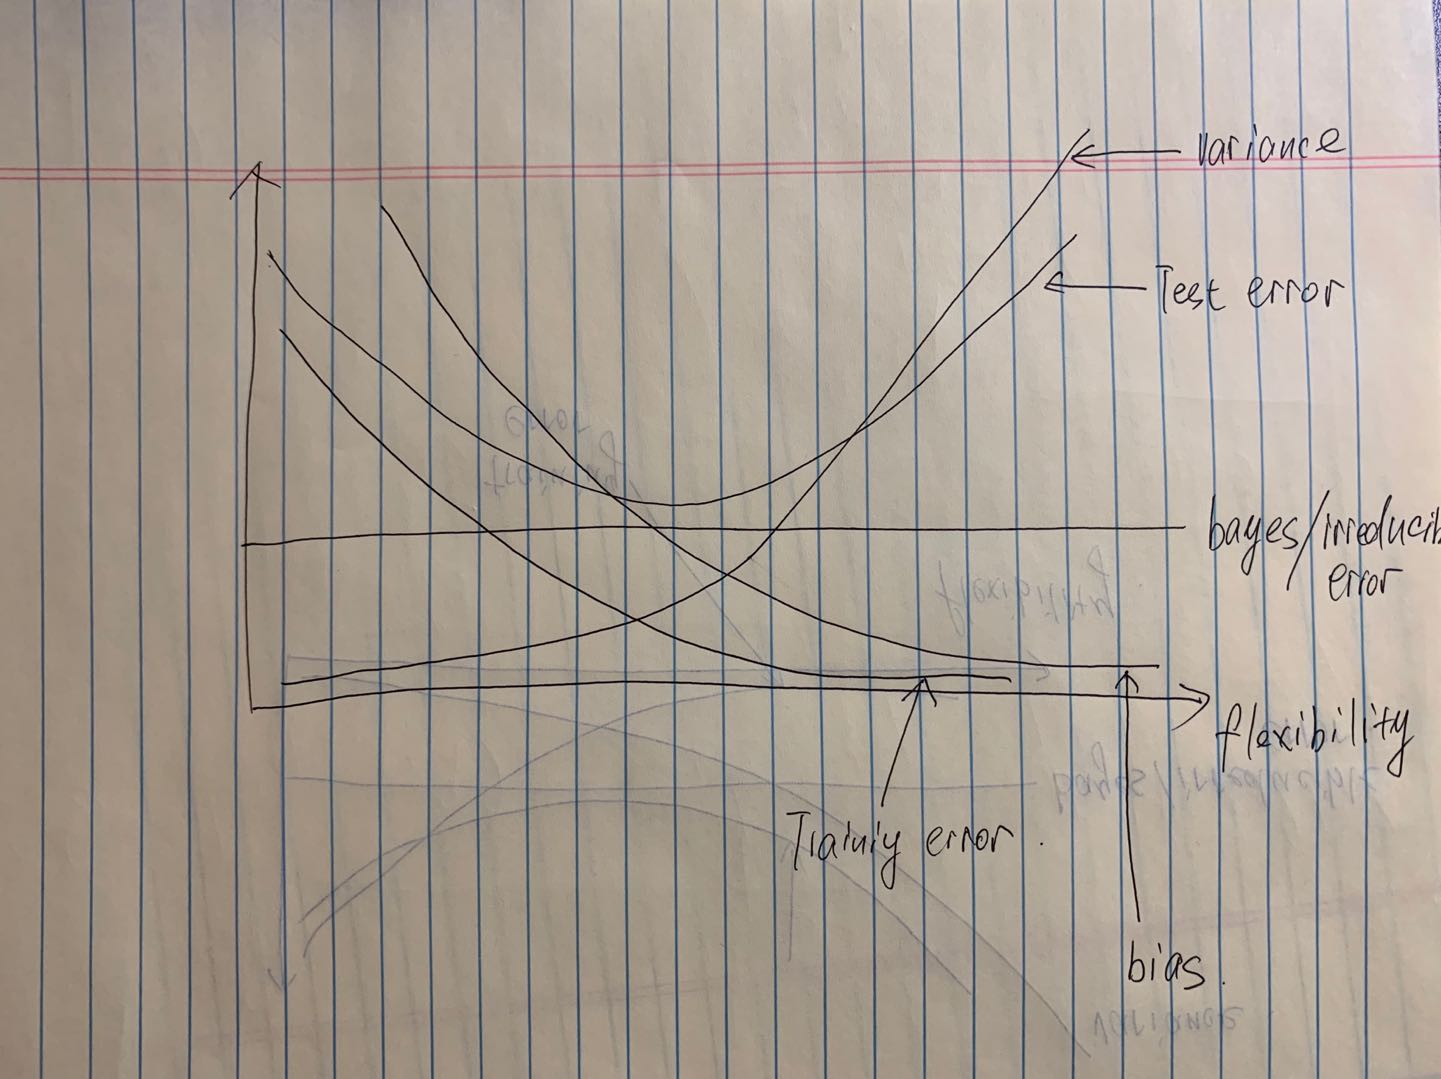
\includegraphics{Chapter2_Exercise3a.png}
\caption{}
\end{figure}

\subsubsection{b)}\label{b-1}

\paragraph{bias:}\label{bias}

Decreases as flexibility increases. Because when the flexibility
increases, the model will fit the data closer, the model will try to fit
the data correctly.

\paragraph{variance:}\label{variance}

Increases as fiexibility increases. Because when the flexibility
increases, the more change with new data.

\paragraph{training error:}\label{training-error}

Decreases as flexibility increases. Because when the flexibility
increases, the model will fit the data closer and more correct.

\paragraph{test error:}\label{test-error}

The shape looks like ``U''. Firstly, test error will decrease with
flexibility, because as flexiblity increases, model will get the correct
trend of fitting data. An appropriate model with test data will make a
great result. However, there is a tipping point, as flexibility
increases, the model will cause overfitting. The model can fit training
data verly close and correct, in this condition, the model only focus on
fit the training data. The model cannot be use for any dataset but the
training data.

\paragraph{bayes/irreducible error:}\label{bayesirreducible-error}

According to the definition, the error is constant.

\subsection{Chapter 2 - Exercise 8}\label{chapter-2---exercise-8}

warnings(`off')

\begin{Shaded}
\begin{Highlighting}[]
\NormalTok{college =}\StringTok{ }\KeywordTok{read.csv}\NormalTok{(}\StringTok{"College.csv"}\NormalTok{)}
\end{Highlighting}
\end{Shaded}

\subsubsection{b)}\label{b-2}

\begin{Shaded}
\begin{Highlighting}[]
\KeywordTok{fix}\NormalTok{(college)}

\KeywordTok{rownames}\NormalTok{(college) =}\StringTok{ }\NormalTok{college[,}\DecValTok{1}\NormalTok{]}
\KeywordTok{fix}\NormalTok{(college)}

\NormalTok{college =}\StringTok{ }\NormalTok{college[,}\OperatorTok{-}\DecValTok{1}\NormalTok{]}
\KeywordTok{fix}\NormalTok{(college)}
\end{Highlighting}
\end{Shaded}

\subsubsection{c)}\label{c-1}

\paragraph{i)}\label{i}

\begin{Shaded}
\begin{Highlighting}[]
\KeywordTok{summary}\NormalTok{(college)}
\end{Highlighting}
\end{Shaded}

\begin{verbatim}
##  Private        Apps           Accept          Enroll       Top10perc    
##  No :212   Min.   :   81   Min.   :   72   Min.   :  35   Min.   : 1.00  
##  Yes:565   1st Qu.:  776   1st Qu.:  604   1st Qu.: 242   1st Qu.:15.00  
##            Median : 1558   Median : 1110   Median : 434   Median :23.00  
##            Mean   : 3002   Mean   : 2019   Mean   : 780   Mean   :27.56  
##            3rd Qu.: 3624   3rd Qu.: 2424   3rd Qu.: 902   3rd Qu.:35.00  
##            Max.   :48094   Max.   :26330   Max.   :6392   Max.   :96.00  
##    Top25perc      F.Undergrad     P.Undergrad         Outstate    
##  Min.   :  9.0   Min.   :  139   Min.   :    1.0   Min.   : 2340  
##  1st Qu.: 41.0   1st Qu.:  992   1st Qu.:   95.0   1st Qu.: 7320  
##  Median : 54.0   Median : 1707   Median :  353.0   Median : 9990  
##  Mean   : 55.8   Mean   : 3700   Mean   :  855.3   Mean   :10441  
##  3rd Qu.: 69.0   3rd Qu.: 4005   3rd Qu.:  967.0   3rd Qu.:12925  
##  Max.   :100.0   Max.   :31643   Max.   :21836.0   Max.   :21700  
##    Room.Board       Books           Personal         PhD        
##  Min.   :1780   Min.   :  96.0   Min.   : 250   Min.   :  8.00  
##  1st Qu.:3597   1st Qu.: 470.0   1st Qu.: 850   1st Qu.: 62.00  
##  Median :4200   Median : 500.0   Median :1200   Median : 75.00  
##  Mean   :4358   Mean   : 549.4   Mean   :1341   Mean   : 72.66  
##  3rd Qu.:5050   3rd Qu.: 600.0   3rd Qu.:1700   3rd Qu.: 85.00  
##  Max.   :8124   Max.   :2340.0   Max.   :6800   Max.   :103.00  
##     Terminal       S.F.Ratio      perc.alumni        Expend     
##  Min.   : 24.0   Min.   : 2.50   Min.   : 0.00   Min.   : 3186  
##  1st Qu.: 71.0   1st Qu.:11.50   1st Qu.:13.00   1st Qu.: 6751  
##  Median : 82.0   Median :13.60   Median :21.00   Median : 8377  
##  Mean   : 79.7   Mean   :14.09   Mean   :22.74   Mean   : 9660  
##  3rd Qu.: 92.0   3rd Qu.:16.50   3rd Qu.:31.00   3rd Qu.:10830  
##  Max.   :100.0   Max.   :39.80   Max.   :64.00   Max.   :56233  
##    Grad.Rate     
##  Min.   : 10.00  
##  1st Qu.: 53.00  
##  Median : 65.00  
##  Mean   : 65.46  
##  3rd Qu.: 78.00  
##  Max.   :118.00
\end{verbatim}

\paragraph{ii)}\label{ii}

\begin{Shaded}
\begin{Highlighting}[]
\KeywordTok{pairs}\NormalTok{(college[,}\DecValTok{1}\OperatorTok{:}\DecValTok{10}\NormalTok{])}
\end{Highlighting}
\end{Shaded}

\includegraphics{Homework1_files/figure-latex/unnamed-chunk-5-1.pdf}

\paragraph{iii)}\label{iii}

\begin{Shaded}
\begin{Highlighting}[]
\KeywordTok{plot}\NormalTok{(college}\OperatorTok{$}\NormalTok{Private,college}\OperatorTok{$}\NormalTok{Outstate)}
\end{Highlighting}
\end{Shaded}

\includegraphics{Homework1_files/figure-latex/unnamed-chunk-6-1.pdf}

\paragraph{iv)}\label{iv}

\begin{Shaded}
\begin{Highlighting}[]
\NormalTok{Elite =}\StringTok{ }\KeywordTok{rep}\NormalTok{(}\StringTok{"No"}\NormalTok{, }\KeywordTok{nrow}\NormalTok{(college))}
\NormalTok{Elite[college}\OperatorTok{$}\NormalTok{Top10perc }\OperatorTok{>}\StringTok{ }\DecValTok{50}\NormalTok{] =}\StringTok{ "Yes"}
\NormalTok{Elite =}\StringTok{ }\KeywordTok{as.factor}\NormalTok{(Elite)}
\NormalTok{college =}\StringTok{ }\KeywordTok{data.frame}\NormalTok{(college , Elite)}

\KeywordTok{summary}\NormalTok{(college)}
\end{Highlighting}
\end{Shaded}

\begin{verbatim}
##  Private        Apps           Accept          Enroll       Top10perc    
##  No :212   Min.   :   81   Min.   :   72   Min.   :  35   Min.   : 1.00  
##  Yes:565   1st Qu.:  776   1st Qu.:  604   1st Qu.: 242   1st Qu.:15.00  
##            Median : 1558   Median : 1110   Median : 434   Median :23.00  
##            Mean   : 3002   Mean   : 2019   Mean   : 780   Mean   :27.56  
##            3rd Qu.: 3624   3rd Qu.: 2424   3rd Qu.: 902   3rd Qu.:35.00  
##            Max.   :48094   Max.   :26330   Max.   :6392   Max.   :96.00  
##    Top25perc      F.Undergrad     P.Undergrad         Outstate    
##  Min.   :  9.0   Min.   :  139   Min.   :    1.0   Min.   : 2340  
##  1st Qu.: 41.0   1st Qu.:  992   1st Qu.:   95.0   1st Qu.: 7320  
##  Median : 54.0   Median : 1707   Median :  353.0   Median : 9990  
##  Mean   : 55.8   Mean   : 3700   Mean   :  855.3   Mean   :10441  
##  3rd Qu.: 69.0   3rd Qu.: 4005   3rd Qu.:  967.0   3rd Qu.:12925  
##  Max.   :100.0   Max.   :31643   Max.   :21836.0   Max.   :21700  
##    Room.Board       Books           Personal         PhD        
##  Min.   :1780   Min.   :  96.0   Min.   : 250   Min.   :  8.00  
##  1st Qu.:3597   1st Qu.: 470.0   1st Qu.: 850   1st Qu.: 62.00  
##  Median :4200   Median : 500.0   Median :1200   Median : 75.00  
##  Mean   :4358   Mean   : 549.4   Mean   :1341   Mean   : 72.66  
##  3rd Qu.:5050   3rd Qu.: 600.0   3rd Qu.:1700   3rd Qu.: 85.00  
##  Max.   :8124   Max.   :2340.0   Max.   :6800   Max.   :103.00  
##     Terminal       S.F.Ratio      perc.alumni        Expend     
##  Min.   : 24.0   Min.   : 2.50   Min.   : 0.00   Min.   : 3186  
##  1st Qu.: 71.0   1st Qu.:11.50   1st Qu.:13.00   1st Qu.: 6751  
##  Median : 82.0   Median :13.60   Median :21.00   Median : 8377  
##  Mean   : 79.7   Mean   :14.09   Mean   :22.74   Mean   : 9660  
##  3rd Qu.: 92.0   3rd Qu.:16.50   3rd Qu.:31.00   3rd Qu.:10830  
##  Max.   :100.0   Max.   :39.80   Max.   :64.00   Max.   :56233  
##    Grad.Rate      Elite    
##  Min.   : 10.00   No :699  
##  1st Qu.: 53.00   Yes: 78  
##  Median : 65.00            
##  Mean   : 65.46            
##  3rd Qu.: 78.00            
##  Max.   :118.00
\end{verbatim}

\begin{Shaded}
\begin{Highlighting}[]
\KeywordTok{plot}\NormalTok{(college}\OperatorTok{$}\NormalTok{Elite, college}\OperatorTok{$}\NormalTok{Outstate)}
\end{Highlighting}
\end{Shaded}

\includegraphics{Homework1_files/figure-latex/unnamed-chunk-7-1.pdf}

There are 78 ``Elite'' colleges and 699 that are not ``Elite.''

\paragraph{v)}\label{v}

\begin{Shaded}
\begin{Highlighting}[]
\KeywordTok{attach}\NormalTok{(college)}
\end{Highlighting}
\end{Shaded}

\begin{verbatim}
## The following object is masked _by_ .GlobalEnv:
## 
##     Elite
\end{verbatim}

\begin{Shaded}
\begin{Highlighting}[]
\KeywordTok{par}\NormalTok{(}\DataTypeTok{mfrow=}\KeywordTok{c}\NormalTok{(}\DecValTok{2}\NormalTok{,}\DecValTok{2}\NormalTok{))}
\KeywordTok{hist}\NormalTok{(Apps, }\DataTypeTok{breaks=}\DecValTok{5}\NormalTok{)}
\KeywordTok{hist}\NormalTok{(Apps, }\DataTypeTok{breaks=}\DecValTok{15}\NormalTok{)}
\KeywordTok{hist}\NormalTok{(Apps, }\DataTypeTok{breaks=}\DecValTok{25}\NormalTok{)}
\KeywordTok{hist}\NormalTok{(Apps, }\DataTypeTok{breaks=}\DecValTok{35}\NormalTok{)}
\end{Highlighting}
\end{Shaded}

\includegraphics{Homework1_files/figure-latex/unnamed-chunk-8-1.pdf}

\begin{Shaded}
\begin{Highlighting}[]
\KeywordTok{par}\NormalTok{(}\DataTypeTok{mfrow=}\KeywordTok{c}\NormalTok{(}\DecValTok{2}\NormalTok{,}\DecValTok{2}\NormalTok{))}
\KeywordTok{hist}\NormalTok{(Accept, }\DataTypeTok{breaks=}\DecValTok{5}\NormalTok{)}
\KeywordTok{hist}\NormalTok{(Accept, }\DataTypeTok{breaks=}\DecValTok{15}\NormalTok{)}
\KeywordTok{hist}\NormalTok{(Accept, }\DataTypeTok{breaks=}\DecValTok{25}\NormalTok{)}
\KeywordTok{hist}\NormalTok{(Accept, }\DataTypeTok{breaks=}\DecValTok{35}\NormalTok{)}
\end{Highlighting}
\end{Shaded}

\includegraphics{Homework1_files/figure-latex/unnamed-chunk-8-2.pdf}

\begin{Shaded}
\begin{Highlighting}[]
\KeywordTok{par}\NormalTok{(}\DataTypeTok{mfrow=}\KeywordTok{c}\NormalTok{(}\DecValTok{2}\NormalTok{,}\DecValTok{2}\NormalTok{))}
\KeywordTok{hist}\NormalTok{(Enroll, }\DataTypeTok{breaks=}\DecValTok{5}\NormalTok{)}
\KeywordTok{hist}\NormalTok{(Enroll, }\DataTypeTok{breaks=}\DecValTok{15}\NormalTok{)}
\KeywordTok{hist}\NormalTok{(Enroll, }\DataTypeTok{breaks=}\DecValTok{25}\NormalTok{)}
\KeywordTok{hist}\NormalTok{(Enroll, }\DataTypeTok{breaks=}\DecValTok{35}\NormalTok{)}
\end{Highlighting}
\end{Shaded}

\includegraphics{Homework1_files/figure-latex/unnamed-chunk-8-3.pdf}

\paragraph{vi)}\label{vi}

\begin{Shaded}
\begin{Highlighting}[]
\KeywordTok{plot}\NormalTok{(college}\OperatorTok{$}\NormalTok{Private,college}\OperatorTok{$}\NormalTok{Books)}
\end{Highlighting}
\end{Shaded}

\includegraphics{Homework1_files/figure-latex/unnamed-chunk-9-1.pdf}

\begin{Shaded}
\begin{Highlighting}[]
\KeywordTok{plot}\NormalTok{(college}\OperatorTok{$}\NormalTok{Elite,college}\OperatorTok{$}\NormalTok{Terminal)}
\end{Highlighting}
\end{Shaded}

\includegraphics{Homework1_files/figure-latex/unnamed-chunk-9-2.pdf}

\begin{Shaded}
\begin{Highlighting}[]
\KeywordTok{plot}\NormalTok{(college}\OperatorTok{$}\NormalTok{Elite,college}\OperatorTok{$}\NormalTok{Grad.Rate)}
\end{Highlighting}
\end{Shaded}

\includegraphics{Homework1_files/figure-latex/unnamed-chunk-9-3.pdf}

\begin{Shaded}
\begin{Highlighting}[]
\KeywordTok{plot}\NormalTok{(college}\OperatorTok{$}\NormalTok{Private,college}\OperatorTok{$}\NormalTok{perc.alumni)}
\end{Highlighting}
\end{Shaded}

\includegraphics{Homework1_files/figure-latex/unnamed-chunk-9-4.pdf}

The median of book costs in private colleges is lower than non-private
colleges.

Obviously, the elite colleges has higher percent of faculty with
terminal degree.And in elite colleges, the percents are very high, the
percents in most elite college are higher than 80\%.

The elite colleges has higher graduation rate, but not higher so much
than non-elite colleges. And there is a unnormal graduation rate in one
of the non-elite colleges.

The private colleges has higher percent of alumni who donate. And the
max donation is much higher than non-private colleges.

\section{Week 2 Exercises}\label{week-2-exercises}

\subsection{Chapter 3 - Exercise 9}\label{chapter-3---exercise-9}

\subsubsection{a)}\label{a-2}

\begin{Shaded}
\begin{Highlighting}[]
\NormalTok{Auto=}\KeywordTok{read.csv}\NormalTok{(}\StringTok{"Auto.csv"}\NormalTok{,}\DataTypeTok{header=}\NormalTok{T,}\DataTypeTok{na.strings =}\StringTok{"?"}\NormalTok{)}

\KeywordTok{pairs}\NormalTok{(Auto)}
\end{Highlighting}
\end{Shaded}

\includegraphics{Homework1_files/figure-latex/unnamed-chunk-10-1.pdf}

\subsubsection{b)}\label{b-3}

\begin{Shaded}
\begin{Highlighting}[]
\KeywordTok{cor}\NormalTok{(Auto[,}\OperatorTok{-}\DecValTok{9}\NormalTok{], }\DataTypeTok{use=}\StringTok{"pairwise.complete.obs"}\NormalTok{)}
\end{Highlighting}
\end{Shaded}

\begin{verbatim}
##                     mpg  cylinders displacement horsepower     weight
## mpg           1.0000000 -0.7762599   -0.8044430 -0.7784268 -0.8317389
## cylinders    -0.7762599  1.0000000    0.9509199  0.8429834  0.8970169
## displacement -0.8044430  0.9509199    1.0000000  0.8972570  0.9331044
## horsepower   -0.7784268  0.8429834    0.8972570  1.0000000  0.8645377
## weight       -0.8317389  0.8970169    0.9331044  0.8645377  1.0000000
## acceleration  0.4222974 -0.5040606   -0.5441618 -0.6891955 -0.4195023
## year          0.5814695 -0.3467172   -0.3698041 -0.4163615 -0.3079004
## origin        0.5636979 -0.5649716   -0.6106643 -0.4551715 -0.5812652
##              acceleration       year     origin
## mpg             0.4222974  0.5814695  0.5636979
## cylinders      -0.5040606 -0.3467172 -0.5649716
## displacement   -0.5441618 -0.3698041 -0.6106643
## horsepower     -0.6891955 -0.4163615 -0.4551715
## weight         -0.4195023 -0.3079004 -0.5812652
## acceleration    1.0000000  0.2829009  0.2100836
## year            0.2829009  1.0000000  0.1843141
## origin          0.2100836  0.1843141  1.0000000
\end{verbatim}

\subsubsection{c)}\label{c-2}

\begin{Shaded}
\begin{Highlighting}[]
\NormalTok{model1 =}\StringTok{ }\KeywordTok{lm}\NormalTok{(mpg }\OperatorTok{~}\StringTok{ }\NormalTok{cylinders }\OperatorTok{+}\StringTok{ }\NormalTok{displacement }\OperatorTok{+}\StringTok{ }\NormalTok{horsepower }\OperatorTok{+}\StringTok{ }\NormalTok{weight }\OperatorTok{+}\StringTok{ }\NormalTok{acceleration }\OperatorTok{+}\StringTok{ }\NormalTok{year }\OperatorTok{+}\StringTok{ }\NormalTok{origin, Auto)}

\KeywordTok{summary}\NormalTok{(model1)}
\end{Highlighting}
\end{Shaded}

\begin{verbatim}
## 
## Call:
## lm(formula = mpg ~ cylinders + displacement + horsepower + weight + 
##     acceleration + year + origin, data = Auto)
## 
## Residuals:
##     Min      1Q  Median      3Q     Max 
## -9.5903 -2.1565 -0.1169  1.8690 13.0604 
## 
## Coefficients:
##                Estimate Std. Error t value Pr(>|t|)    
## (Intercept)  -17.218435   4.644294  -3.707  0.00024 ***
## cylinders     -0.493376   0.323282  -1.526  0.12780    
## displacement   0.019896   0.007515   2.647  0.00844 ** 
## horsepower    -0.016951   0.013787  -1.230  0.21963    
## weight        -0.006474   0.000652  -9.929  < 2e-16 ***
## acceleration   0.080576   0.098845   0.815  0.41548    
## year           0.750773   0.050973  14.729  < 2e-16 ***
## origin         1.426141   0.278136   5.127 4.67e-07 ***
## ---
## Signif. codes:  0 '***' 0.001 '**' 0.01 '*' 0.05 '.' 0.1 ' ' 1
## 
## Residual standard error: 3.328 on 384 degrees of freedom
##   (5 observations deleted due to missingness)
## Multiple R-squared:  0.8215, Adjusted R-squared:  0.8182 
## F-statistic: 252.4 on 7 and 384 DF,  p-value: < 2.2e-16
\end{verbatim}

\paragraph{i)}\label{i-1}

The F-statistic is 224.5,and P value is 2.2e-16. With the aloha level of
0.05, we can conclude that there is a relationship between the
predictors and the cars' mpg.

\paragraph{ii)}\label{ii-1}

Based on the p-values associated with each variable, at an alpha level
of 0.05, all predictors except for cylinders, horsepower and
acceleration had a statistically significant relationship to mpg as last
predictors in.

\paragraph{iii)}\label{iii-1}

The cofficient of year is approximate 0.777, that means when the year
increases 1 year, the mpg will increase 0.777.

\subsubsection{d)}\label{d-1}

\begin{Shaded}
\begin{Highlighting}[]
\KeywordTok{plot}\NormalTok{(model1)}
\end{Highlighting}
\end{Shaded}

\includegraphics{Homework1_files/figure-latex/unnamed-chunk-13-1.pdf}
\includegraphics{Homework1_files/figure-latex/unnamed-chunk-13-2.pdf}
\includegraphics{Homework1_files/figure-latex/unnamed-chunk-13-3.pdf}
\includegraphics{Homework1_files/figure-latex/unnamed-chunk-13-4.pdf}

Based on the Residuals vs Fitted plot, there looks like a curves
relationship between the fitted values and residuals.That means linear
regression may not be appropriate for the data.

Look at Normal Q-Q plot, there is a observation much higher. That means
this observation 323 may have unnormal value.

According to the Residuals vs Leverage plot, there are no individual
data points with unusually high leverage.

\subsubsection{e)}\label{e}

\begin{Shaded}
\begin{Highlighting}[]
\NormalTok{model2 =}\StringTok{ }\KeywordTok{lm}\NormalTok{(mpg }\OperatorTok{~}\StringTok{ }\NormalTok{cylinders }\OperatorTok{*}\StringTok{ }\NormalTok{displacement }\OperatorTok{*}\StringTok{ }\NormalTok{horsepower }\OperatorTok{*}\StringTok{ }\NormalTok{weight }\OperatorTok{*}\StringTok{ }\NormalTok{acceleration }\OperatorTok{*}\StringTok{ }\NormalTok{year }\OperatorTok{*}\StringTok{ }\NormalTok{origin, Auto)}
\KeywordTok{anova}\NormalTok{(model1, model2)}
\end{Highlighting}
\end{Shaded}

\begin{verbatim}
## Analysis of Variance Table
## 
## Model 1: mpg ~ cylinders + displacement + horsepower + weight + acceleration + 
##     year + origin
## Model 2: mpg ~ cylinders * displacement * horsepower * weight * acceleration * 
##     year * origin
##   Res.Df    RSS  Df Sum of Sq      F    Pr(>F)    
## 1    384 4252.2                                   
## 2    279 1631.2 105      2621 4.2695 < 2.2e-16 ***
## ---
## Signif. codes:  0 '***' 0.001 '**' 0.01 '*' 0.05 '.' 0.1 ' ' 1
\end{verbatim}

\begin{Shaded}
\begin{Highlighting}[]
\NormalTok{model3 =}\StringTok{ }\KeywordTok{lm}\NormalTok{(mpg }\OperatorTok{~}\StringTok{ }\NormalTok{cylinders }\OperatorTok{:}\StringTok{ }\NormalTok{displacement }\OperatorTok{:}\StringTok{ }\NormalTok{horsepower }\OperatorTok{:}\StringTok{ }\NormalTok{weight }\OperatorTok{*}\StringTok{ }\NormalTok{acceleration }\OperatorTok{:}\StringTok{ }\NormalTok{year }\OperatorTok{:}\StringTok{ }\NormalTok{origin, Auto)}
\KeywordTok{anova}\NormalTok{(model1, model3)}
\end{Highlighting}
\end{Shaded}

\begin{verbatim}
## Analysis of Variance Table
## 
## Model 1: mpg ~ cylinders + displacement + horsepower + weight + acceleration + 
##     year + origin
## Model 2: mpg ~ cylinders:displacement:horsepower:weight * acceleration:year:origin
##   Res.Df    RSS Df Sum of Sq      F    Pr(>F)    
## 1    384 4252.2                                  
## 2    388 7913.3 -4   -3661.1 82.655 < 2.2e-16 ***
## ---
## Signif. codes:  0 '***' 0.001 '**' 0.01 '*' 0.05 '.' 0.1 ' ' 1
\end{verbatim}

According to the low P value, there are statistically significant
interactions between the predictor variables.

\paragraph{f)}\label{f}

\begin{Shaded}
\begin{Highlighting}[]
\NormalTok{Auto}\OperatorTok{$}\NormalTok{displacement.t =}\StringTok{ }\KeywordTok{log}\NormalTok{(Auto}\OperatorTok{$}\NormalTok{displacement)}
\NormalTok{Auto}\OperatorTok{$}\NormalTok{horsepower.t =}\StringTok{ }\KeywordTok{log}\NormalTok{(Auto}\OperatorTok{$}\NormalTok{horsepower)}
\NormalTok{Auto}\OperatorTok{$}\NormalTok{weight.t =}\StringTok{ }\KeywordTok{log}\NormalTok{(Auto}\OperatorTok{$}\NormalTok{weight)}
\NormalTok{Auto}\OperatorTok{$}\NormalTok{year.t =}\StringTok{ }\KeywordTok{log}\NormalTok{(Auto}\OperatorTok{$}\NormalTok{year)}

\NormalTok{model_log =}\StringTok{ }\KeywordTok{lm}\NormalTok{(mpg }\OperatorTok{~}\StringTok{ }\NormalTok{cylinders }\OperatorTok{*}\StringTok{ }\NormalTok{displacement.t }\OperatorTok{*}\StringTok{ }\NormalTok{horsepower.t }\OperatorTok{*}\StringTok{ }\NormalTok{weight.t }\OperatorTok{*}\StringTok{ }\NormalTok{acceleration }\OperatorTok{*}\StringTok{ }\NormalTok{year.t }\OperatorTok{*}\StringTok{ }\NormalTok{origin, Auto)}
\KeywordTok{plot}\NormalTok{(model_log)}
\end{Highlighting}
\end{Shaded}

\begin{verbatim}
## Warning: not plotting observations with leverage one:
##   71, 111, 123, 209, 210, 240, 242, 274, 276, 296, 326, 331, 332, 356, 357, 358
\end{verbatim}

\includegraphics{Homework1_files/figure-latex/unnamed-chunk-16-1.pdf}
\includegraphics{Homework1_files/figure-latex/unnamed-chunk-16-2.pdf}

\begin{verbatim}
## Warning: not plotting observations with leverage one:
##   71, 111, 123, 209, 210, 240, 242, 274, 276, 296, 326, 331, 332, 356, 357, 358
\end{verbatim}

\includegraphics{Homework1_files/figure-latex/unnamed-chunk-16-3.pdf}

\begin{verbatim}
## Warning in sqrt(crit * p * (1 - hh)/hh): 产生了NaNs
\end{verbatim}

\begin{verbatim}
## Warning in sqrt(crit * p * (1 - hh)/hh): 产生了NaNs
\end{verbatim}

\includegraphics{Homework1_files/figure-latex/unnamed-chunk-16-4.pdf}

Using log transformation, the Residuals vs Fitted plot, the relationship
looks like more appropriate, and there are some high-leverage points.

\begin{Shaded}
\begin{Highlighting}[]
\NormalTok{Auto}\OperatorTok{$}\NormalTok{cylinders.tt =}\StringTok{ }\NormalTok{(Auto}\OperatorTok{$}\NormalTok{cylinders)}\OperatorTok{^}\DecValTok{2}
\NormalTok{Auto}\OperatorTok{$}\NormalTok{acceleration.tt =}\StringTok{ }\NormalTok{(Auto}\OperatorTok{$}\NormalTok{acceleration)}\OperatorTok{^}\DecValTok{2}

\NormalTok{model.}\DecValTok{2}\NormalTok{ =}\StringTok{ }\KeywordTok{lm}\NormalTok{(mpg }\OperatorTok{~}\StringTok{ }\NormalTok{cylinders.tt }\OperatorTok{*}\StringTok{ }\NormalTok{displacement }\OperatorTok{*}\StringTok{ }\NormalTok{horsepower }\OperatorTok{*}\StringTok{ }\NormalTok{weight }\OperatorTok{*}\StringTok{ }\NormalTok{acceleration.tt }\OperatorTok{*}\StringTok{ }\NormalTok{year }\OperatorTok{*}\StringTok{ }\NormalTok{origin, Auto)}
\KeywordTok{plot}\NormalTok{(model.}\DecValTok{2}\NormalTok{)}
\end{Highlighting}
\end{Shaded}

\begin{verbatim}
## Warning: not plotting observations with leverage one:
##   71, 111, 123, 209, 210, 240, 242, 273, 274, 276, 296, 326, 331, 332, 356, 357, 358
\end{verbatim}

\includegraphics{Homework1_files/figure-latex/unnamed-chunk-17-1.pdf}
\includegraphics{Homework1_files/figure-latex/unnamed-chunk-17-2.pdf}

\begin{verbatim}
## Warning: not plotting observations with leverage one:
##   71, 111, 123, 209, 210, 240, 242, 273, 274, 276, 296, 326, 331, 332, 356, 357, 358
\end{verbatim}

\includegraphics{Homework1_files/figure-latex/unnamed-chunk-17-3.pdf}

\begin{verbatim}
## Warning in sqrt(crit * p * (1 - hh)/hh): 产生了NaNs
\end{verbatim}

\begin{verbatim}
## Warning in sqrt(crit * p * (1 - hh)/hh): 产生了NaNs
\end{verbatim}

\includegraphics{Homework1_files/figure-latex/unnamed-chunk-17-4.pdf}

Using log transformation, there are some high-leverage points.

\section{Chapter 3 - Exercise 15}\label{chapter-3---exercise-15}

\begin{Shaded}
\begin{Highlighting}[]
\KeywordTok{library}\NormalTok{(MASS)}
\end{Highlighting}
\end{Shaded}

\begin{Shaded}
\begin{Highlighting}[]
\NormalTok{model.zn =}\StringTok{ }\KeywordTok{lm}\NormalTok{(crim }\OperatorTok{~}\StringTok{ }\NormalTok{zn, Boston)}
\NormalTok{model.indus =}\StringTok{ }\KeywordTok{lm}\NormalTok{(crim }\OperatorTok{~}\StringTok{ }\NormalTok{indus, Boston)}
\NormalTok{model.chas =}\StringTok{ }\KeywordTok{lm}\NormalTok{(crim }\OperatorTok{~}\StringTok{ }\NormalTok{chas, Boston)}
\NormalTok{model.nox =}\StringTok{ }\KeywordTok{lm}\NormalTok{(crim }\OperatorTok{~}\StringTok{ }\NormalTok{nox, Boston)}
\NormalTok{model.rm =}\StringTok{ }\KeywordTok{lm}\NormalTok{(crim }\OperatorTok{~}\StringTok{ }\NormalTok{rm, Boston)}
\NormalTok{model.age =}\StringTok{ }\KeywordTok{lm}\NormalTok{(crim }\OperatorTok{~}\StringTok{ }\NormalTok{age, Boston)}
\NormalTok{model.dis =}\StringTok{ }\KeywordTok{lm}\NormalTok{(crim }\OperatorTok{~}\StringTok{ }\NormalTok{dis, Boston)}
\NormalTok{model.rad =}\StringTok{ }\KeywordTok{lm}\NormalTok{(crim }\OperatorTok{~}\StringTok{ }\NormalTok{rad, Boston)}
\NormalTok{model.tax =}\StringTok{ }\KeywordTok{lm}\NormalTok{(crim }\OperatorTok{~}\StringTok{ }\NormalTok{tax, Boston)}
\NormalTok{model.ptratio =}\StringTok{ }\KeywordTok{lm}\NormalTok{(crim }\OperatorTok{~}\StringTok{ }\NormalTok{ptratio, Boston)}
\NormalTok{model.black =}\StringTok{ }\KeywordTok{lm}\NormalTok{(crim }\OperatorTok{~}\StringTok{ }\NormalTok{black, Boston)}
\NormalTok{model.lstat =}\StringTok{ }\KeywordTok{lm}\NormalTok{(crim }\OperatorTok{~}\StringTok{ }\NormalTok{lstat, Boston)}
\NormalTok{model.medv =}\StringTok{ }\KeywordTok{lm}\NormalTok{(crim }\OperatorTok{~}\StringTok{ }\NormalTok{medv, Boston)}

\KeywordTok{summary}\NormalTok{(model.zn)}
\end{Highlighting}
\end{Shaded}

\begin{verbatim}
## 
## Call:
## lm(formula = crim ~ zn, data = Boston)
## 
## Residuals:
##    Min     1Q Median     3Q    Max 
## -4.429 -4.222 -2.620  1.250 84.523 
## 
## Coefficients:
##             Estimate Std. Error t value Pr(>|t|)    
## (Intercept)  4.45369    0.41722  10.675  < 2e-16 ***
## zn          -0.07393    0.01609  -4.594 5.51e-06 ***
## ---
## Signif. codes:  0 '***' 0.001 '**' 0.01 '*' 0.05 '.' 0.1 ' ' 1
## 
## Residual standard error: 8.435 on 504 degrees of freedom
## Multiple R-squared:  0.04019,    Adjusted R-squared:  0.03828 
## F-statistic:  21.1 on 1 and 504 DF,  p-value: 5.506e-06
\end{verbatim}

\begin{Shaded}
\begin{Highlighting}[]
\KeywordTok{summary}\NormalTok{(model.indus)}
\end{Highlighting}
\end{Shaded}

\begin{verbatim}
## 
## Call:
## lm(formula = crim ~ indus, data = Boston)
## 
## Residuals:
##     Min      1Q  Median      3Q     Max 
## -11.972  -2.698  -0.736   0.712  81.813 
## 
## Coefficients:
##             Estimate Std. Error t value Pr(>|t|)    
## (Intercept) -2.06374    0.66723  -3.093  0.00209 ** 
## indus        0.50978    0.05102   9.991  < 2e-16 ***
## ---
## Signif. codes:  0 '***' 0.001 '**' 0.01 '*' 0.05 '.' 0.1 ' ' 1
## 
## Residual standard error: 7.866 on 504 degrees of freedom
## Multiple R-squared:  0.1653, Adjusted R-squared:  0.1637 
## F-statistic: 99.82 on 1 and 504 DF,  p-value: < 2.2e-16
\end{verbatim}

\begin{Shaded}
\begin{Highlighting}[]
\KeywordTok{summary}\NormalTok{(model.chas)}
\end{Highlighting}
\end{Shaded}

\begin{verbatim}
## 
## Call:
## lm(formula = crim ~ chas, data = Boston)
## 
## Residuals:
##    Min     1Q Median     3Q    Max 
## -3.738 -3.661 -3.435  0.018 85.232 
## 
## Coefficients:
##             Estimate Std. Error t value Pr(>|t|)    
## (Intercept)   3.7444     0.3961   9.453   <2e-16 ***
## chas         -1.8928     1.5061  -1.257    0.209    
## ---
## Signif. codes:  0 '***' 0.001 '**' 0.01 '*' 0.05 '.' 0.1 ' ' 1
## 
## Residual standard error: 8.597 on 504 degrees of freedom
## Multiple R-squared:  0.003124,   Adjusted R-squared:  0.001146 
## F-statistic: 1.579 on 1 and 504 DF,  p-value: 0.2094
\end{verbatim}

\begin{Shaded}
\begin{Highlighting}[]
\KeywordTok{summary}\NormalTok{(model.nox)}
\end{Highlighting}
\end{Shaded}

\begin{verbatim}
## 
## Call:
## lm(formula = crim ~ nox, data = Boston)
## 
## Residuals:
##     Min      1Q  Median      3Q     Max 
## -12.371  -2.738  -0.974   0.559  81.728 
## 
## Coefficients:
##             Estimate Std. Error t value Pr(>|t|)    
## (Intercept)  -13.720      1.699  -8.073 5.08e-15 ***
## nox           31.249      2.999  10.419  < 2e-16 ***
## ---
## Signif. codes:  0 '***' 0.001 '**' 0.01 '*' 0.05 '.' 0.1 ' ' 1
## 
## Residual standard error: 7.81 on 504 degrees of freedom
## Multiple R-squared:  0.1772, Adjusted R-squared:  0.1756 
## F-statistic: 108.6 on 1 and 504 DF,  p-value: < 2.2e-16
\end{verbatim}

\begin{Shaded}
\begin{Highlighting}[]
\KeywordTok{summary}\NormalTok{(model.rm)}
\end{Highlighting}
\end{Shaded}

\begin{verbatim}
## 
## Call:
## lm(formula = crim ~ rm, data = Boston)
## 
## Residuals:
##    Min     1Q Median     3Q    Max 
## -6.604 -3.952 -2.654  0.989 87.197 
## 
## Coefficients:
##             Estimate Std. Error t value Pr(>|t|)    
## (Intercept)   20.482      3.365   6.088 2.27e-09 ***
## rm            -2.684      0.532  -5.045 6.35e-07 ***
## ---
## Signif. codes:  0 '***' 0.001 '**' 0.01 '*' 0.05 '.' 0.1 ' ' 1
## 
## Residual standard error: 8.401 on 504 degrees of freedom
## Multiple R-squared:  0.04807,    Adjusted R-squared:  0.04618 
## F-statistic: 25.45 on 1 and 504 DF,  p-value: 6.347e-07
\end{verbatim}

\begin{Shaded}
\begin{Highlighting}[]
\KeywordTok{summary}\NormalTok{(model.age)}
\end{Highlighting}
\end{Shaded}

\begin{verbatim}
## 
## Call:
## lm(formula = crim ~ age, data = Boston)
## 
## Residuals:
##    Min     1Q Median     3Q    Max 
## -6.789 -4.257 -1.230  1.527 82.849 
## 
## Coefficients:
##             Estimate Std. Error t value Pr(>|t|)    
## (Intercept) -3.77791    0.94398  -4.002 7.22e-05 ***
## age          0.10779    0.01274   8.463 2.85e-16 ***
## ---
## Signif. codes:  0 '***' 0.001 '**' 0.01 '*' 0.05 '.' 0.1 ' ' 1
## 
## Residual standard error: 8.057 on 504 degrees of freedom
## Multiple R-squared:  0.1244, Adjusted R-squared:  0.1227 
## F-statistic: 71.62 on 1 and 504 DF,  p-value: 2.855e-16
\end{verbatim}

\begin{Shaded}
\begin{Highlighting}[]
\KeywordTok{summary}\NormalTok{(model.dis)}
\end{Highlighting}
\end{Shaded}

\begin{verbatim}
## 
## Call:
## lm(formula = crim ~ dis, data = Boston)
## 
## Residuals:
##    Min     1Q Median     3Q    Max 
## -6.708 -4.134 -1.527  1.516 81.674 
## 
## Coefficients:
##             Estimate Std. Error t value Pr(>|t|)    
## (Intercept)   9.4993     0.7304  13.006   <2e-16 ***
## dis          -1.5509     0.1683  -9.213   <2e-16 ***
## ---
## Signif. codes:  0 '***' 0.001 '**' 0.01 '*' 0.05 '.' 0.1 ' ' 1
## 
## Residual standard error: 7.965 on 504 degrees of freedom
## Multiple R-squared:  0.1441, Adjusted R-squared:  0.1425 
## F-statistic: 84.89 on 1 and 504 DF,  p-value: < 2.2e-16
\end{verbatim}

\begin{Shaded}
\begin{Highlighting}[]
\KeywordTok{summary}\NormalTok{(model.rad)}
\end{Highlighting}
\end{Shaded}

\begin{verbatim}
## 
## Call:
## lm(formula = crim ~ rad, data = Boston)
## 
## Residuals:
##     Min      1Q  Median      3Q     Max 
## -10.164  -1.381  -0.141   0.660  76.433 
## 
## Coefficients:
##             Estimate Std. Error t value Pr(>|t|)    
## (Intercept) -2.28716    0.44348  -5.157 3.61e-07 ***
## rad          0.61791    0.03433  17.998  < 2e-16 ***
## ---
## Signif. codes:  0 '***' 0.001 '**' 0.01 '*' 0.05 '.' 0.1 ' ' 1
## 
## Residual standard error: 6.718 on 504 degrees of freedom
## Multiple R-squared:  0.3913, Adjusted R-squared:   0.39 
## F-statistic: 323.9 on 1 and 504 DF,  p-value: < 2.2e-16
\end{verbatim}

\begin{Shaded}
\begin{Highlighting}[]
\KeywordTok{summary}\NormalTok{(model.tax)}
\end{Highlighting}
\end{Shaded}

\begin{verbatim}
## 
## Call:
## lm(formula = crim ~ tax, data = Boston)
## 
## Residuals:
##     Min      1Q  Median      3Q     Max 
## -12.513  -2.738  -0.194   1.065  77.696 
## 
## Coefficients:
##              Estimate Std. Error t value Pr(>|t|)    
## (Intercept) -8.528369   0.815809  -10.45   <2e-16 ***
## tax          0.029742   0.001847   16.10   <2e-16 ***
## ---
## Signif. codes:  0 '***' 0.001 '**' 0.01 '*' 0.05 '.' 0.1 ' ' 1
## 
## Residual standard error: 6.997 on 504 degrees of freedom
## Multiple R-squared:  0.3396, Adjusted R-squared:  0.3383 
## F-statistic: 259.2 on 1 and 504 DF,  p-value: < 2.2e-16
\end{verbatim}

\begin{Shaded}
\begin{Highlighting}[]
\KeywordTok{summary}\NormalTok{(model.ptratio)}
\end{Highlighting}
\end{Shaded}

\begin{verbatim}
## 
## Call:
## lm(formula = crim ~ ptratio, data = Boston)
## 
## Residuals:
##    Min     1Q Median     3Q    Max 
## -7.654 -3.985 -1.912  1.825 83.353 
## 
## Coefficients:
##             Estimate Std. Error t value Pr(>|t|)    
## (Intercept) -17.6469     3.1473  -5.607 3.40e-08 ***
## ptratio       1.1520     0.1694   6.801 2.94e-11 ***
## ---
## Signif. codes:  0 '***' 0.001 '**' 0.01 '*' 0.05 '.' 0.1 ' ' 1
## 
## Residual standard error: 8.24 on 504 degrees of freedom
## Multiple R-squared:  0.08407,    Adjusted R-squared:  0.08225 
## F-statistic: 46.26 on 1 and 504 DF,  p-value: 2.943e-11
\end{verbatim}

\begin{Shaded}
\begin{Highlighting}[]
\KeywordTok{summary}\NormalTok{(model.black)}
\end{Highlighting}
\end{Shaded}

\begin{verbatim}
## 
## Call:
## lm(formula = crim ~ black, data = Boston)
## 
## Residuals:
##     Min      1Q  Median      3Q     Max 
## -13.756  -2.299  -2.095  -1.296  86.822 
## 
## Coefficients:
##              Estimate Std. Error t value Pr(>|t|)    
## (Intercept) 16.553529   1.425903  11.609   <2e-16 ***
## black       -0.036280   0.003873  -9.367   <2e-16 ***
## ---
## Signif. codes:  0 '***' 0.001 '**' 0.01 '*' 0.05 '.' 0.1 ' ' 1
## 
## Residual standard error: 7.946 on 504 degrees of freedom
## Multiple R-squared:  0.1483, Adjusted R-squared:  0.1466 
## F-statistic: 87.74 on 1 and 504 DF,  p-value: < 2.2e-16
\end{verbatim}

\begin{Shaded}
\begin{Highlighting}[]
\KeywordTok{summary}\NormalTok{(model.lstat)}
\end{Highlighting}
\end{Shaded}

\begin{verbatim}
## 
## Call:
## lm(formula = crim ~ lstat, data = Boston)
## 
## Residuals:
##     Min      1Q  Median      3Q     Max 
## -13.925  -2.822  -0.664   1.079  82.862 
## 
## Coefficients:
##             Estimate Std. Error t value Pr(>|t|)    
## (Intercept) -3.33054    0.69376  -4.801 2.09e-06 ***
## lstat        0.54880    0.04776  11.491  < 2e-16 ***
## ---
## Signif. codes:  0 '***' 0.001 '**' 0.01 '*' 0.05 '.' 0.1 ' ' 1
## 
## Residual standard error: 7.664 on 504 degrees of freedom
## Multiple R-squared:  0.2076, Adjusted R-squared:  0.206 
## F-statistic:   132 on 1 and 504 DF,  p-value: < 2.2e-16
\end{verbatim}

\begin{Shaded}
\begin{Highlighting}[]
\KeywordTok{summary}\NormalTok{(model.medv)}
\end{Highlighting}
\end{Shaded}

\begin{verbatim}
## 
## Call:
## lm(formula = crim ~ medv, data = Boston)
## 
## Residuals:
##    Min     1Q Median     3Q    Max 
## -9.071 -4.022 -2.343  1.298 80.957 
## 
## Coefficients:
##             Estimate Std. Error t value Pr(>|t|)    
## (Intercept) 11.79654    0.93419   12.63   <2e-16 ***
## medv        -0.36316    0.03839   -9.46   <2e-16 ***
## ---
## Signif. codes:  0 '***' 0.001 '**' 0.01 '*' 0.05 '.' 0.1 ' ' 1
## 
## Residual standard error: 7.934 on 504 degrees of freedom
## Multiple R-squared:  0.1508, Adjusted R-squared:  0.1491 
## F-statistic: 89.49 on 1 and 504 DF,  p-value: < 2.2e-16
\end{verbatim}

According to the P values of all models, all variables are statistically
significant predictors of crim, except for chas.

\begin{Shaded}
\begin{Highlighting}[]
\KeywordTok{plot}\NormalTok{(Boston}\OperatorTok{$}\NormalTok{zn, Boston}\OperatorTok{$}\NormalTok{crim)}
\end{Highlighting}
\end{Shaded}

\includegraphics{Homework1_files/figure-latex/unnamed-chunk-19-1.pdf}

\begin{Shaded}
\begin{Highlighting}[]
\KeywordTok{plot}\NormalTok{(Boston}\OperatorTok{$}\NormalTok{indus, Boston}\OperatorTok{$}\NormalTok{crim)}
\end{Highlighting}
\end{Shaded}

\includegraphics{Homework1_files/figure-latex/unnamed-chunk-20-1.pdf}

\begin{Shaded}
\begin{Highlighting}[]
\KeywordTok{plot}\NormalTok{(Boston}\OperatorTok{$}\NormalTok{chas, Boston}\OperatorTok{$}\NormalTok{crim)}
\end{Highlighting}
\end{Shaded}

\includegraphics{Homework1_files/figure-latex/unnamed-chunk-21-1.pdf}

\begin{Shaded}
\begin{Highlighting}[]
\KeywordTok{plot}\NormalTok{(Boston}\OperatorTok{$}\NormalTok{nox, Boston}\OperatorTok{$}\NormalTok{crim)}
\end{Highlighting}
\end{Shaded}

\includegraphics{Homework1_files/figure-latex/unnamed-chunk-22-1.pdf}

\begin{Shaded}
\begin{Highlighting}[]
\KeywordTok{plot}\NormalTok{(Boston}\OperatorTok{$}\NormalTok{rm, Boston}\OperatorTok{$}\NormalTok{crim)}
\end{Highlighting}
\end{Shaded}

\includegraphics{Homework1_files/figure-latex/unnamed-chunk-23-1.pdf}

\begin{Shaded}
\begin{Highlighting}[]
\KeywordTok{plot}\NormalTok{(Boston}\OperatorTok{$}\NormalTok{age, Boston}\OperatorTok{$}\NormalTok{crim)}
\end{Highlighting}
\end{Shaded}

\includegraphics{Homework1_files/figure-latex/unnamed-chunk-24-1.pdf}

\begin{Shaded}
\begin{Highlighting}[]
\KeywordTok{plot}\NormalTok{(Boston}\OperatorTok{$}\NormalTok{dis, Boston}\OperatorTok{$}\NormalTok{crim)}
\end{Highlighting}
\end{Shaded}

\includegraphics{Homework1_files/figure-latex/unnamed-chunk-25-1.pdf}

\begin{Shaded}
\begin{Highlighting}[]
\KeywordTok{plot}\NormalTok{(Boston}\OperatorTok{$}\NormalTok{rad, Boston}\OperatorTok{$}\NormalTok{crim)}
\end{Highlighting}
\end{Shaded}

\includegraphics{Homework1_files/figure-latex/unnamed-chunk-26-1.pdf}

\begin{Shaded}
\begin{Highlighting}[]
\KeywordTok{plot}\NormalTok{(Boston}\OperatorTok{$}\NormalTok{tax, Boston}\OperatorTok{$}\NormalTok{crim)}
\end{Highlighting}
\end{Shaded}

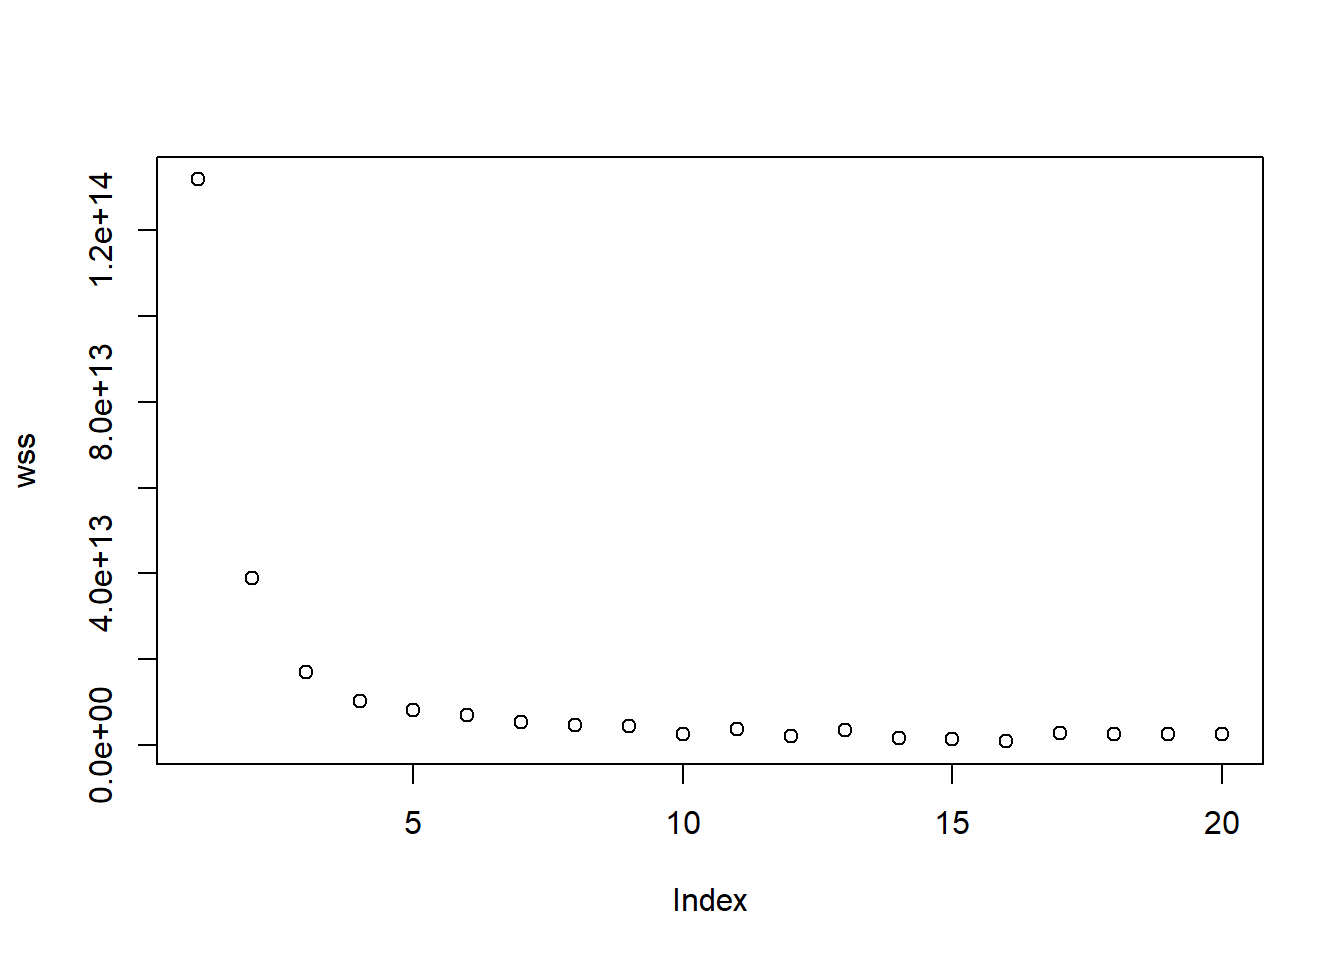
\includegraphics{Homework1_files/figure-latex/unnamed-chunk-27-1.pdf}

\begin{Shaded}
\begin{Highlighting}[]
\KeywordTok{plot}\NormalTok{(Boston}\OperatorTok{$}\NormalTok{ptratio, Boston}\OperatorTok{$}\NormalTok{crim)}
\end{Highlighting}
\end{Shaded}

\includegraphics{Homework1_files/figure-latex/unnamed-chunk-28-1.pdf}

\begin{Shaded}
\begin{Highlighting}[]
\KeywordTok{plot}\NormalTok{(Boston}\OperatorTok{$}\NormalTok{black, Boston}\OperatorTok{$}\NormalTok{crim)}
\end{Highlighting}
\end{Shaded}

\includegraphics{Homework1_files/figure-latex/unnamed-chunk-29-1.pdf}

\begin{Shaded}
\begin{Highlighting}[]
\KeywordTok{plot}\NormalTok{(Boston}\OperatorTok{$}\NormalTok{lstat, Boston}\OperatorTok{$}\NormalTok{crim)}
\end{Highlighting}
\end{Shaded}

\includegraphics{Homework1_files/figure-latex/unnamed-chunk-30-1.pdf}

\begin{Shaded}
\begin{Highlighting}[]
\KeywordTok{plot}\NormalTok{(Boston}\OperatorTok{$}\NormalTok{medv, Boston}\OperatorTok{$}\NormalTok{crim)}
\end{Highlighting}
\end{Shaded}

\includegraphics{Homework1_files/figure-latex/unnamed-chunk-31-1.pdf}

\subsubsection{b)}\label{b-4}

\begin{Shaded}
\begin{Highlighting}[]
\NormalTok{model_b =}\StringTok{ }\KeywordTok{lm}\NormalTok{(crim }\OperatorTok{~}\StringTok{ }\NormalTok{zn }\OperatorTok{+}\StringTok{ }\NormalTok{indus }\OperatorTok{+}\StringTok{ }\NormalTok{chas }\OperatorTok{+}\StringTok{ }\NormalTok{nox }\OperatorTok{+}\StringTok{ }\NormalTok{rm }\OperatorTok{+}\StringTok{ }\NormalTok{age }\OperatorTok{+}\StringTok{ }\NormalTok{dis }\OperatorTok{+}\StringTok{ }\NormalTok{rad }\OperatorTok{+}\StringTok{ }\NormalTok{tax }\OperatorTok{+}\StringTok{ }\NormalTok{ptratio }\OperatorTok{+}\StringTok{ }\NormalTok{black }\OperatorTok{+}\StringTok{ }\NormalTok{lstat }\OperatorTok{+}\StringTok{ }\NormalTok{medv, Boston)}
\KeywordTok{summary}\NormalTok{(model_b)}
\end{Highlighting}
\end{Shaded}

\begin{verbatim}
## 
## Call:
## lm(formula = crim ~ zn + indus + chas + nox + rm + age + dis + 
##     rad + tax + ptratio + black + lstat + medv, data = Boston)
## 
## Residuals:
##    Min     1Q Median     3Q    Max 
## -9.924 -2.120 -0.353  1.019 75.051 
## 
## Coefficients:
##               Estimate Std. Error t value Pr(>|t|)    
## (Intercept)  17.033228   7.234903   2.354 0.018949 *  
## zn            0.044855   0.018734   2.394 0.017025 *  
## indus        -0.063855   0.083407  -0.766 0.444294    
## chas         -0.749134   1.180147  -0.635 0.525867    
## nox         -10.313535   5.275536  -1.955 0.051152 .  
## rm            0.430131   0.612830   0.702 0.483089    
## age           0.001452   0.017925   0.081 0.935488    
## dis          -0.987176   0.281817  -3.503 0.000502 ***
## rad           0.588209   0.088049   6.680 6.46e-11 ***
## tax          -0.003780   0.005156  -0.733 0.463793    
## ptratio      -0.271081   0.186450  -1.454 0.146611    
## black        -0.007538   0.003673  -2.052 0.040702 *  
## lstat         0.126211   0.075725   1.667 0.096208 .  
## medv         -0.198887   0.060516  -3.287 0.001087 ** 
## ---
## Signif. codes:  0 '***' 0.001 '**' 0.01 '*' 0.05 '.' 0.1 ' ' 1
## 
## Residual standard error: 6.439 on 492 degrees of freedom
## Multiple R-squared:  0.454,  Adjusted R-squared:  0.4396 
## F-statistic: 31.47 on 13 and 492 DF,  p-value: < 2.2e-16
\end{verbatim}

If the alpha level is 0.05, we can reject the null hypothesis for the
predictors: zn,dis,rad,black and medv. The P-value of these predictors
are lower than 0.05.

\subsubsection{c)}\label{c-3}

\begin{Shaded}
\begin{Highlighting}[]
\NormalTok{simple.coefficients =}\StringTok{ }\KeywordTok{c}\NormalTok{(}\KeywordTok{coefficients}\NormalTok{(model.zn)[}\DecValTok{2}\NormalTok{], }\KeywordTok{coefficients}\NormalTok{(model.indus)[}\DecValTok{2}\NormalTok{],}
                        \KeywordTok{coefficients}\NormalTok{(model.chas)[}\DecValTok{2}\NormalTok{], }\KeywordTok{coefficients}\NormalTok{(model.nox)[}\DecValTok{2}\NormalTok{],}
                        \KeywordTok{coefficients}\NormalTok{(model.rm)[}\DecValTok{2}\NormalTok{], }\KeywordTok{coefficients}\NormalTok{(model.age)[}\DecValTok{2}\NormalTok{],}
                        \KeywordTok{coefficients}\NormalTok{(model.dis)[}\DecValTok{2}\NormalTok{], }\KeywordTok{coefficients}\NormalTok{(model.rad)[}\DecValTok{2}\NormalTok{],}
                        \KeywordTok{coefficients}\NormalTok{(model.tax)[}\DecValTok{2}\NormalTok{], }\KeywordTok{coefficients}\NormalTok{(model.ptratio)[}\DecValTok{2}\NormalTok{],}
                        \KeywordTok{coefficients}\NormalTok{(model.black)[}\DecValTok{2}\NormalTok{], }\KeywordTok{coefficients}\NormalTok{(model.lstat)[}\DecValTok{2}\NormalTok{],}
                        \KeywordTok{coefficients}\NormalTok{(model.medv)[}\DecValTok{2}\NormalTok{])}
\NormalTok{multiple.coefficients =}\StringTok{ }\KeywordTok{coefficients}\NormalTok{(model_b)[}\DecValTok{2}\OperatorTok{:}\DecValTok{14}\NormalTok{]}
\KeywordTok{plot}\NormalTok{(simple.coefficients, multiple.coefficients)}
\end{Highlighting}
\end{Shaded}

\includegraphics{Homework1_files/figure-latex/unnamed-chunk-33-1.pdf}

All the variable are clustered in the top left corner, except one
variable. Let's find which variable is so special:

\begin{Shaded}
\begin{Highlighting}[]
\NormalTok{simple.coefficients}
\end{Highlighting}
\end{Shaded}

\begin{verbatim}
##          zn       indus        chas         nox          rm         age 
## -0.07393498  0.50977633 -1.89277655 31.24853120 -2.68405122  0.10778623 
##         dis         rad         tax     ptratio       black       lstat 
## -1.55090168  0.61791093  0.02974225  1.15198279 -0.03627964  0.54880478 
##        medv 
## -0.36315992
\end{verbatim}

The variable in the bottom right corner is nox.

\subsubsection{d)}\label{d-2}

\begin{Shaded}
\begin{Highlighting}[]
\NormalTok{model.zn.nonlinear =}\StringTok{ }\KeywordTok{lm}\NormalTok{(crim }\OperatorTok{~}\StringTok{ }\KeywordTok{poly}\NormalTok{(zn, }\DecValTok{3}\NormalTok{), Boston)}
\NormalTok{model.indus.nonlinear =}\StringTok{ }\KeywordTok{lm}\NormalTok{(crim }\OperatorTok{~}\StringTok{ }\KeywordTok{poly}\NormalTok{(indus, }\DecValTok{3}\NormalTok{), Boston)}
\NormalTok{model.chas.nonlinear =}\StringTok{ }\KeywordTok{lm}\NormalTok{(crim }\OperatorTok{~}\StringTok{ }\NormalTok{chas }\OperatorTok{+}\StringTok{ }\KeywordTok{I}\NormalTok{(chas}\OperatorTok{^}\DecValTok{2}\NormalTok{) }\OperatorTok{+}\StringTok{ }\KeywordTok{I}\NormalTok{(chas}\OperatorTok{^}\DecValTok{3}\NormalTok{), Boston)}
\NormalTok{model.nox.nonlinear =}\StringTok{ }\KeywordTok{lm}\NormalTok{(crim }\OperatorTok{~}\StringTok{ }\KeywordTok{poly}\NormalTok{(nox, }\DecValTok{3}\NormalTok{), Boston)}
\NormalTok{model.rm.nonlinear =}\StringTok{ }\KeywordTok{lm}\NormalTok{(crim }\OperatorTok{~}\StringTok{ }\KeywordTok{poly}\NormalTok{(rm, }\DecValTok{3}\NormalTok{), Boston)}
\NormalTok{model.age.nonlinear =}\StringTok{ }\KeywordTok{lm}\NormalTok{(crim }\OperatorTok{~}\StringTok{ }\KeywordTok{poly}\NormalTok{(age, }\DecValTok{3}\NormalTok{), Boston)}
\NormalTok{model.dis.nonlinear =}\StringTok{ }\KeywordTok{lm}\NormalTok{(crim }\OperatorTok{~}\StringTok{ }\KeywordTok{poly}\NormalTok{(dis, }\DecValTok{3}\NormalTok{), Boston)}
\NormalTok{model.rad.nonlinear =}\StringTok{ }\KeywordTok{lm}\NormalTok{(crim }\OperatorTok{~}\StringTok{ }\KeywordTok{poly}\NormalTok{(rad, }\DecValTok{3}\NormalTok{), Boston)}
\NormalTok{model.tax.nonlinear =}\StringTok{ }\KeywordTok{lm}\NormalTok{(crim }\OperatorTok{~}\StringTok{ }\KeywordTok{poly}\NormalTok{(tax, }\DecValTok{3}\NormalTok{), Boston)}
\NormalTok{model.ptratio.nonlinear =}\StringTok{ }\KeywordTok{lm}\NormalTok{(crim }\OperatorTok{~}\StringTok{ }\KeywordTok{poly}\NormalTok{(ptratio, }\DecValTok{3}\NormalTok{), Boston)}
\NormalTok{model.black.nonlinear =}\StringTok{ }\KeywordTok{lm}\NormalTok{(crim }\OperatorTok{~}\StringTok{ }\KeywordTok{poly}\NormalTok{(black, }\DecValTok{3}\NormalTok{), Boston)}
\NormalTok{model.lstat.nonlinear =}\StringTok{ }\KeywordTok{lm}\NormalTok{(crim }\OperatorTok{~}\StringTok{ }\KeywordTok{poly}\NormalTok{(lstat, }\DecValTok{3}\NormalTok{), Boston)}
\NormalTok{model.medv.nonlinear =}\StringTok{ }\KeywordTok{lm}\NormalTok{(crim }\OperatorTok{~}\StringTok{ }\KeywordTok{poly}\NormalTok{(medv, }\DecValTok{3}\NormalTok{), Boston)}

\KeywordTok{anova}\NormalTok{(model.zn, model.zn.nonlinear)}
\end{Highlighting}
\end{Shaded}

\begin{verbatim}
## Analysis of Variance Table
## 
## Model 1: crim ~ zn
## Model 2: crim ~ poly(zn, 3)
##   Res.Df   RSS Df Sum of Sq      F   Pr(>F)   
## 1    504 35862                                
## 2    502 35187  2    674.56 4.8118 0.008512 **
## ---
## Signif. codes:  0 '***' 0.001 '**' 0.01 '*' 0.05 '.' 0.1 ' ' 1
\end{verbatim}

\begin{Shaded}
\begin{Highlighting}[]
\KeywordTok{anova}\NormalTok{(model.indus, model.indus.nonlinear)}
\end{Highlighting}
\end{Shaded}

\begin{verbatim}
## Analysis of Variance Table
## 
## Model 1: crim ~ indus
## Model 2: crim ~ poly(indus, 3)
##   Res.Df   RSS Df Sum of Sq      F    Pr(>F)    
## 1    504 31187                                  
## 2    502 27662  2    3525.1 31.987 8.409e-14 ***
## ---
## Signif. codes:  0 '***' 0.001 '**' 0.01 '*' 0.05 '.' 0.1 ' ' 1
\end{verbatim}

\begin{Shaded}
\begin{Highlighting}[]
\KeywordTok{anova}\NormalTok{(model.chas, model.chas.nonlinear)}
\end{Highlighting}
\end{Shaded}

\begin{verbatim}
## Analysis of Variance Table
## 
## Model 1: crim ~ chas
## Model 2: crim ~ chas + I(chas^2) + I(chas^3)
##   Res.Df   RSS Df Sum of Sq F Pr(>F)
## 1    504 37247                      
## 2    504 37247  0         0
\end{verbatim}

\begin{Shaded}
\begin{Highlighting}[]
\KeywordTok{anova}\NormalTok{(model.nox, model.nox.nonlinear)}
\end{Highlighting}
\end{Shaded}

\begin{verbatim}
## Analysis of Variance Table
## 
## Model 1: crim ~ nox
## Model 2: crim ~ poly(nox, 3)
##   Res.Df   RSS Df Sum of Sq      F    Pr(>F)    
## 1    504 30742                                  
## 2    502 26267  2    4474.6 42.758 < 2.2e-16 ***
## ---
## Signif. codes:  0 '***' 0.001 '**' 0.01 '*' 0.05 '.' 0.1 ' ' 1
\end{verbatim}

\begin{Shaded}
\begin{Highlighting}[]
\KeywordTok{anova}\NormalTok{(model.rm, model.rm.nonlinear)}
\end{Highlighting}
\end{Shaded}

\begin{verbatim}
## Analysis of Variance Table
## 
## Model 1: crim ~ rm
## Model 2: crim ~ poly(rm, 3)
##   Res.Df   RSS Df Sum of Sq      F   Pr(>F)   
## 1    504 35567                                
## 2    502 34831  2    736.69 5.3088 0.005229 **
## ---
## Signif. codes:  0 '***' 0.001 '**' 0.01 '*' 0.05 '.' 0.1 ' ' 1
\end{verbatim}

\begin{Shaded}
\begin{Highlighting}[]
\KeywordTok{anova}\NormalTok{(model.age, model.age.nonlinear)}
\end{Highlighting}
\end{Shaded}

\begin{verbatim}
## Analysis of Variance Table
## 
## Model 1: crim ~ age
## Model 2: crim ~ poly(age, 3)
##   Res.Df   RSS Df Sum of Sq     F    Pr(>F)    
## 1    504 32714                                 
## 2    502 30853  2      1861 15.14 4.125e-07 ***
## ---
## Signif. codes:  0 '***' 0.001 '**' 0.01 '*' 0.05 '.' 0.1 ' ' 1
\end{verbatim}

\begin{Shaded}
\begin{Highlighting}[]
\KeywordTok{anova}\NormalTok{(model.dis, model.dis.nonlinear)}
\end{Highlighting}
\end{Shaded}

\begin{verbatim}
## Analysis of Variance Table
## 
## Model 1: crim ~ dis
## Model 2: crim ~ poly(dis, 3)
##   Res.Df   RSS Df Sum of Sq     F    Pr(>F)    
## 1    504 31977                                 
## 2    502 26983  2    4994.5 46.46 < 2.2e-16 ***
## ---
## Signif. codes:  0 '***' 0.001 '**' 0.01 '*' 0.05 '.' 0.1 ' ' 1
\end{verbatim}

\begin{Shaded}
\begin{Highlighting}[]
\KeywordTok{anova}\NormalTok{(model.rad, model.rad.nonlinear)}
\end{Highlighting}
\end{Shaded}

\begin{verbatim}
## Analysis of Variance Table
## 
## Model 1: crim ~ rad
## Model 2: crim ~ poly(rad, 3)
##   Res.Df   RSS Df Sum of Sq      F  Pr(>F)  
## 1    504 22745                              
## 2    502 22417  2    328.06 3.6733 0.02608 *
## ---
## Signif. codes:  0 '***' 0.001 '**' 0.01 '*' 0.05 '.' 0.1 ' ' 1
\end{verbatim}

\begin{Shaded}
\begin{Highlighting}[]
\KeywordTok{anova}\NormalTok{(model.tax, model.tax.nonlinear)}
\end{Highlighting}
\end{Shaded}

\begin{verbatim}
## Analysis of Variance Table
## 
## Model 1: crim ~ tax
## Model 2: crim ~ poly(tax, 3)
##   Res.Df   RSS Df Sum of Sq     F    Pr(>F)    
## 1    504 24674                                 
## 2    502 23581  2    1093.5 11.64 1.144e-05 ***
## ---
## Signif. codes:  0 '***' 0.001 '**' 0.01 '*' 0.05 '.' 0.1 ' ' 1
\end{verbatim}

\begin{Shaded}
\begin{Highlighting}[]
\KeywordTok{anova}\NormalTok{(model.ptratio, model.ptratio.nonlinear)}
\end{Highlighting}
\end{Shaded}

\begin{verbatim}
## Analysis of Variance Table
## 
## Model 1: crim ~ ptratio
## Model 2: crim ~ poly(ptratio, 3)
##   Res.Df   RSS Df Sum of Sq      F    Pr(>F)    
## 1    504 34222                                  
## 2    502 33112  2    1110.2 8.4155 0.0002542 ***
## ---
## Signif. codes:  0 '***' 0.001 '**' 0.01 '*' 0.05 '.' 0.1 ' ' 1
\end{verbatim}

\begin{Shaded}
\begin{Highlighting}[]
\KeywordTok{anova}\NormalTok{(model.black, model.black.nonlinear)}
\end{Highlighting}
\end{Shaded}

\begin{verbatim}
## Analysis of Variance Table
## 
## Model 1: crim ~ black
## Model 2: crim ~ poly(black, 3)
##   Res.Df   RSS Df Sum of Sq      F Pr(>F)
## 1    504 31823                           
## 2    502 31765  2    58.495 0.4622 0.6302
\end{verbatim}

\begin{Shaded}
\begin{Highlighting}[]
\KeywordTok{anova}\NormalTok{(model.lstat, model.lstat.nonlinear)}
\end{Highlighting}
\end{Shaded}

\begin{verbatim}
## Analysis of Variance Table
## 
## Model 1: crim ~ lstat
## Model 2: crim ~ poly(lstat, 3)
##   Res.Df   RSS Df Sum of Sq     F  Pr(>F)  
## 1    504 29607                             
## 2    502 29221  2    386.39 3.319 0.03698 *
## ---
## Signif. codes:  0 '***' 0.001 '**' 0.01 '*' 0.05 '.' 0.1 ' ' 1
\end{verbatim}

\begin{Shaded}
\begin{Highlighting}[]
\KeywordTok{anova}\NormalTok{(model.medv, model.medv.nonlinear)}
\end{Highlighting}
\end{Shaded}

\begin{verbatim}
## Analysis of Variance Table
## 
## Model 1: crim ~ medv
## Model 2: crim ~ poly(medv, 3)
##   Res.Df   RSS Df Sum of Sq      F    Pr(>F)    
## 1    504 31730                                  
## 2    502 21663  2     10066 116.63 < 2.2e-16 ***
## ---
## Signif. codes:  0 '***' 0.001 '**' 0.01 '*' 0.05 '.' 0.1 ' ' 1
\end{verbatim}

If the alpha level is 0.05, the polynomial transformation of all
predictor variables generate better models except for chas and black.
Because chas is a binary variable, transformation won't change the
model.So we can conclude that these predictor variables may have
non-linear relationship with crim.

\section{Week 3 Homework}\label{week-3-homework}

\subsection{Chapter 4 - Exercise 13}\label{chapter-4---exercise-13}

\subsubsection{logistic regression}\label{logistic-regression}

\begin{Shaded}
\begin{Highlighting}[]
\KeywordTok{median}\NormalTok{(Boston}\OperatorTok{$}\NormalTok{crim)}
\end{Highlighting}
\end{Shaded}

\begin{verbatim}
## [1] 0.25651
\end{verbatim}

\begin{Shaded}
\begin{Highlighting}[]
\NormalTok{Boston}\OperatorTok{$}\NormalTok{crim.higher.median =}\StringTok{ }\KeywordTok{ifelse}\NormalTok{(Boston}\OperatorTok{$}\NormalTok{crim }\OperatorTok{>=}\StringTok{ }\KeywordTok{median}\NormalTok{(Boston}\OperatorTok{$}\NormalTok{crim), }\DecValTok{1}\NormalTok{, }\DecValTok{0}\NormalTok{)}
\end{Highlighting}
\end{Shaded}

\begin{Shaded}
\begin{Highlighting}[]
\NormalTok{train =}\StringTok{ }\DecValTok{1}\OperatorTok{:}\NormalTok{(}\KeywordTok{dim}\NormalTok{(Boston)[}\DecValTok{1}\NormalTok{]}\OperatorTok{*}\NormalTok{.}\DecValTok{8}\NormalTok{)}
\NormalTok{test =}\StringTok{ }\NormalTok{(}\KeywordTok{dim}\NormalTok{(Boston)[}\DecValTok{1}\NormalTok{]}\OperatorTok{*}\NormalTok{.}\DecValTok{8} \OperatorTok{+}\StringTok{ }\NormalTok{.}\DecValTok{1}\NormalTok{)}\OperatorTok{:}\KeywordTok{dim}\NormalTok{(Boston)[}\DecValTok{1}\NormalTok{]}

\NormalTok{Boston.train =}\StringTok{ }\NormalTok{Boston[train,]}
\NormalTok{Boston.test =}\StringTok{ }\NormalTok{Boston[test,]}
\end{Highlighting}
\end{Shaded}

\begin{Shaded}
\begin{Highlighting}[]
\NormalTok{log_reg =}\StringTok{ }\KeywordTok{glm}\NormalTok{((crim.higher.median }\OperatorTok{==}\StringTok{ }\DecValTok{1}\NormalTok{) }\OperatorTok{~}\StringTok{ }\NormalTok{zn }\OperatorTok{+}\StringTok{ }\NormalTok{indus }\OperatorTok{+}\StringTok{ }\NormalTok{chas }\OperatorTok{+}\StringTok{ }\NormalTok{nox }\OperatorTok{+}\StringTok{ }\NormalTok{rm }\OperatorTok{+}\StringTok{ }\NormalTok{age }\OperatorTok{+}\StringTok{ }\NormalTok{dis }\OperatorTok{+}\StringTok{ }\NormalTok{rad }\OperatorTok{+}\StringTok{ }\NormalTok{tax }\OperatorTok{+}\StringTok{ }\NormalTok{ptratio }\OperatorTok{+}\StringTok{ }\NormalTok{black }\OperatorTok{+}\StringTok{ }\NormalTok{lstat }\OperatorTok{+}\StringTok{ }\NormalTok{medv, }\DataTypeTok{data=}\NormalTok{Boston.train, }\DataTypeTok{family=}\NormalTok{binomial)}
\KeywordTok{summary}\NormalTok{(log_reg)}
\end{Highlighting}
\end{Shaded}

\begin{verbatim}
## 
## Call:
## glm(formula = (crim.higher.median == 1) ~ zn + indus + chas + 
##     nox + rm + age + dis + rad + tax + ptratio + black + lstat + 
##     medv, family = binomial, data = Boston.train)
## 
## Deviance Residuals: 
##     Min       1Q   Median       3Q      Max  
## -2.3643  -0.2023  -0.0140   0.0725   3.4545  
## 
## Coefficients:
##               Estimate Std. Error z value Pr(>|z|)    
## (Intercept) -42.799126   7.890654  -5.424 5.83e-08 ***
## zn           -0.066836   0.036978  -1.807 0.070693 .  
## indus        -0.088478   0.051755  -1.710 0.087348 .  
## chas          1.023592   0.753024   1.359 0.174049    
## nox          59.170895   9.555418   6.192 5.93e-10 ***
## rm           -0.676176   0.816094  -0.829 0.407358    
## age           0.008651   0.012974   0.667 0.504913    
## dis           0.654216   0.232581   2.813 0.004910 ** 
## rad           0.621347   0.183645   3.383 0.000716 ***
## tax          -0.001433   0.003760  -0.381 0.703173    
## ptratio       0.485265   0.141219   3.436 0.000590 ***
## black        -0.009549   0.006112  -1.562 0.118192    
## lstat         0.068709   0.054149   1.269 0.204480    
## medv          0.202732   0.080269   2.526 0.011548 *  
## ---
## Signif. codes:  0 '***' 0.001 '**' 0.01 '*' 0.05 '.' 0.1 ' ' 1
## 
## (Dispersion parameter for binomial family taken to be 1)
## 
##     Null deviance: 547.16  on 403  degrees of freedom
## Residual deviance: 182.50  on 390  degrees of freedom
## AIC: 210.5
## 
## Number of Fisher Scoring iterations: 9
\end{verbatim}

\begin{Shaded}
\begin{Highlighting}[]
\NormalTok{log.reg.probabilities =}\StringTok{ }\KeywordTok{predict}\NormalTok{(log_reg, Boston.test, }\DataTypeTok{type=}\StringTok{"response"}\NormalTok{)}
\NormalTok{log.reg.predictions =}\StringTok{ }\KeywordTok{ifelse}\NormalTok{(log.reg.probabilities }\OperatorTok{>=}\StringTok{ }\FloatTok{0.5}\NormalTok{, }\DecValTok{1}\NormalTok{, }\DecValTok{0}\NormalTok{)}
\KeywordTok{mean}\NormalTok{(log.reg.predictions }\OperatorTok{!=}\StringTok{ }\NormalTok{Boston.test}\OperatorTok{$}\NormalTok{crim.higher.median)}
\end{Highlighting}
\end{Shaded}

\begin{verbatim}
## [1] 0.09803922
\end{verbatim}

The error rate on this test sample is 9.8\%.

Now, we use the statistically significant predictors(nox,rad,ptratio and
medv) to generate a model.

\begin{Shaded}
\begin{Highlighting}[]
\NormalTok{log_reg2 =}\StringTok{ }\KeywordTok{glm}\NormalTok{((crim.higher.median }\OperatorTok{==}\StringTok{ }\DecValTok{1}\NormalTok{) }\OperatorTok{~}\StringTok{ }\NormalTok{nox }\OperatorTok{+}\StringTok{ }\NormalTok{dis }\OperatorTok{+}\StringTok{ }\NormalTok{rad }\OperatorTok{+}\StringTok{ }\NormalTok{ptratio }\OperatorTok{+}\StringTok{ }\NormalTok{medv, }\DataTypeTok{data=}\NormalTok{Boston.train, }\DataTypeTok{family=}\NormalTok{binomial)}
\KeywordTok{summary}\NormalTok{(log_reg2)}
\end{Highlighting}
\end{Shaded}

\begin{verbatim}
## 
## Call:
## glm(formula = (crim.higher.median == 1) ~ nox + dis + rad + ptratio + 
##     medv, family = binomial, data = Boston.train)
## 
## Deviance Residuals: 
##      Min        1Q    Median        3Q       Max  
## -2.78458  -0.27292  -0.07535   0.09379   3.02537  
## 
## Coefficients:
##              Estimate Std. Error z value Pr(>|z|)    
## (Intercept) -42.01873    6.37902  -6.587 4.49e-11 ***
## nox          51.59479    7.57454   6.812 9.65e-12 ***
## dis           0.31550    0.15899   1.984 0.047202 *  
## rad           0.59144    0.13470   4.391 1.13e-05 ***
## ptratio       0.45053    0.11738   3.838 0.000124 ***
## medv          0.09295    0.03264   2.847 0.004407 ** 
## ---
## Signif. codes:  0 '***' 0.001 '**' 0.01 '*' 0.05 '.' 0.1 ' ' 1
## 
## (Dispersion parameter for binomial family taken to be 1)
## 
##     Null deviance: 547.16  on 403  degrees of freedom
## Residual deviance: 200.32  on 398  degrees of freedom
## AIC: 212.32
## 
## Number of Fisher Scoring iterations: 8
\end{verbatim}

\begin{Shaded}
\begin{Highlighting}[]
\NormalTok{log.reg.probabilities2 =}\StringTok{ }\KeywordTok{predict}\NormalTok{(log_reg2, Boston.test, }\DataTypeTok{type=}\StringTok{"response"}\NormalTok{)}
\NormalTok{log.reg.predictions2 =}\StringTok{ }\KeywordTok{ifelse}\NormalTok{(log.reg.probabilities2 }\OperatorTok{>=}\StringTok{ }\FloatTok{0.5}\NormalTok{, }\DecValTok{1}\NormalTok{, }\DecValTok{0}\NormalTok{)}
\KeywordTok{mean}\NormalTok{(log.reg.predictions2 }\OperatorTok{!=}\StringTok{ }\NormalTok{Boston.test}\OperatorTok{$}\NormalTok{crim.higher.median)}
\end{Highlighting}
\end{Shaded}

\begin{verbatim}
## [1] 0.1372549
\end{verbatim}

Well,according to the error rate, the model is worse.

\subsubsection{LDA}\label{lda}

\begin{Shaded}
\begin{Highlighting}[]
\NormalTok{lda1 =}\StringTok{ }\KeywordTok{lda}\NormalTok{((crim.higher.median }\OperatorTok{==}\StringTok{ }\DecValTok{1}\NormalTok{) }\OperatorTok{~}\StringTok{ }\NormalTok{zn }\OperatorTok{+}\StringTok{ }\NormalTok{indus }\OperatorTok{+}\StringTok{ }\NormalTok{chas }\OperatorTok{+}\StringTok{ }\NormalTok{nox }\OperatorTok{+}\StringTok{ }\NormalTok{rm }\OperatorTok{+}\StringTok{ }\NormalTok{age }\OperatorTok{+}\StringTok{ }\NormalTok{dis }\OperatorTok{+}\StringTok{ }\NormalTok{rad }\OperatorTok{+}\StringTok{ }\NormalTok{tax }\OperatorTok{+}\StringTok{ }\NormalTok{ptratio }\OperatorTok{+}\StringTok{ }\NormalTok{black }\OperatorTok{+}\StringTok{ }\NormalTok{lstat }\OperatorTok{+}\StringTok{ }\NormalTok{medv, }\DataTypeTok{data=}\NormalTok{Boston.train)}

\NormalTok{lda.predictions.text1 =}\StringTok{ }\KeywordTok{predict}\NormalTok{(lda1, Boston.test)}
\NormalTok{lda.predictions1 =}\StringTok{ }\KeywordTok{ifelse}\NormalTok{(lda.predictions.text1}\OperatorTok{$}\NormalTok{class }\OperatorTok{==}\StringTok{ "TRUE"}\NormalTok{, }\DecValTok{1}\NormalTok{, }\DecValTok{0}\NormalTok{)}

\KeywordTok{mean}\NormalTok{(lda.predictions1 }\OperatorTok{!=}\StringTok{ }\NormalTok{Boston.test}\OperatorTok{$}\NormalTok{crim.higher.median)}
\end{Highlighting}
\end{Shaded}

\begin{verbatim}
## [1] 0.127451
\end{verbatim}

The error rate on this test sample is 12.7\%.

\begin{Shaded}
\begin{Highlighting}[]
\NormalTok{lda2 =}\StringTok{ }\KeywordTok{lda}\NormalTok{((crim.higher.median }\OperatorTok{==}\StringTok{ }\DecValTok{1}\NormalTok{) }\OperatorTok{~}\StringTok{ }\NormalTok{nox }\OperatorTok{+}\StringTok{ }\NormalTok{dis }\OperatorTok{+}\StringTok{ }\NormalTok{rad }\OperatorTok{+}\StringTok{ }\NormalTok{ptratio }\OperatorTok{+}\StringTok{ }\NormalTok{medv, }\DataTypeTok{data=}\NormalTok{Boston.train)}

\NormalTok{lda.predictions.text2 =}\StringTok{ }\KeywordTok{predict}\NormalTok{(lda2, Boston.test)}
\NormalTok{lda.predictions2 =}\StringTok{ }\KeywordTok{ifelse}\NormalTok{(lda.predictions.text2}\OperatorTok{$}\NormalTok{class }\OperatorTok{==}\StringTok{ "TRUE"}\NormalTok{, }\DecValTok{1}\NormalTok{, }\DecValTok{0}\NormalTok{)}

\KeywordTok{mean}\NormalTok{(lda.predictions2 }\OperatorTok{!=}\StringTok{ }\NormalTok{Boston.test}\OperatorTok{$}\NormalTok{crim.higher.median)}
\end{Highlighting}
\end{Shaded}

\begin{verbatim}
## [1] 0.1372549
\end{verbatim}

For LDA, using statistically significant predictors also creates a worse
medel.

\subsubsection{KNN}\label{knn}

\begin{Shaded}
\begin{Highlighting}[]
\KeywordTok{library}\NormalTok{(class)}
\NormalTok{train.X =}\StringTok{ }\KeywordTok{cbind}\NormalTok{(Boston.train}\OperatorTok{$}\NormalTok{zn, Boston.train}\OperatorTok{$}\NormalTok{indus, Boston.train}\OperatorTok{$}\NormalTok{chas, Boston.train}\OperatorTok{$}\NormalTok{nox, }
\NormalTok{                Boston.train}\OperatorTok{$}\NormalTok{rm, Boston.train}\OperatorTok{$}\NormalTok{age, Boston.train}\OperatorTok{$}\NormalTok{dis, Boston.train}\OperatorTok{$}\NormalTok{rad, }
\NormalTok{                Boston.train}\OperatorTok{$}\NormalTok{tax, Boston.train}\OperatorTok{$}\NormalTok{ptratio, Boston.train}\OperatorTok{$}\NormalTok{black, }
\NormalTok{                Boston.train}\OperatorTok{$}\NormalTok{lstat, Boston.train}\OperatorTok{$}\NormalTok{medv)}
\NormalTok{test.X  =}\StringTok{ }\KeywordTok{cbind}\NormalTok{(Boston.test}\OperatorTok{$}\NormalTok{zn, Boston.test}\OperatorTok{$}\NormalTok{indus, Boston.test}\OperatorTok{$}\NormalTok{chas, Boston.test}\OperatorTok{$}\NormalTok{nox, }
\NormalTok{                Boston.test}\OperatorTok{$}\NormalTok{rm, Boston.test}\OperatorTok{$}\NormalTok{age, Boston.test}\OperatorTok{$}\NormalTok{dis, Boston.test}\OperatorTok{$}\NormalTok{rad, }
\NormalTok{                Boston.test}\OperatorTok{$}\NormalTok{tax, Boston.test}\OperatorTok{$}\NormalTok{ptratio, Boston.test}\OperatorTok{$}\NormalTok{black, Boston.test}\OperatorTok{$}\NormalTok{lstat, }
\NormalTok{                Boston.test}\OperatorTok{$}\NormalTok{medv)}

\NormalTok{train.X2 =}\StringTok{ }\KeywordTok{cbind}\NormalTok{(Boston.train}\OperatorTok{$}\NormalTok{nox, Boston.train}\OperatorTok{$}\NormalTok{dis, Boston.train}\OperatorTok{$}\NormalTok{rad, }
\NormalTok{                 Boston.train}\OperatorTok{$}\NormalTok{ptratio,Boston.train}\OperatorTok{$}\NormalTok{medv)}
\NormalTok{test.X2  =}\StringTok{ }\KeywordTok{cbind}\NormalTok{(Boston.test}\OperatorTok{$}\NormalTok{nox, Boston.test}\OperatorTok{$}\NormalTok{dis, Boston.test}\OperatorTok{$}\NormalTok{rad, }
\NormalTok{                 Boston.test}\OperatorTok{$}\NormalTok{ptratio,Boston.test}\OperatorTok{$}\NormalTok{medv)}
\end{Highlighting}
\end{Shaded}

\begin{Shaded}
\begin{Highlighting}[]
\KeywordTok{set.seed}\NormalTok{(}\DecValTok{0}\NormalTok{)}
\NormalTok{knn1 =}\StringTok{ }\KeywordTok{knn}\NormalTok{(train.X, test.X, Boston.train}\OperatorTok{$}\NormalTok{crim.higher.median, }\DataTypeTok{k =} \DecValTok{10}\NormalTok{)}
\KeywordTok{mean}\NormalTok{(knn1 }\OperatorTok{!=}\StringTok{ }\NormalTok{Boston.test}\OperatorTok{$}\NormalTok{crim.higher.median)}
\end{Highlighting}
\end{Shaded}

\begin{verbatim}
## [1] 0.07843137
\end{verbatim}

The error rate of KNN method with K=10 is only 7.8\%.

\begin{Shaded}
\begin{Highlighting}[]
\KeywordTok{set.seed}\NormalTok{(}\DecValTok{1}\NormalTok{)}
\NormalTok{knn2 =}\StringTok{ }\KeywordTok{knn}\NormalTok{(train.X2, test.X2, Boston.train}\OperatorTok{$}\NormalTok{crim.higher.median, }\DataTypeTok{k =} \DecValTok{10}\NormalTok{)}

\KeywordTok{mean}\NormalTok{(knn2 }\OperatorTok{!=}\StringTok{ }\NormalTok{Boston.test}\OperatorTok{$}\NormalTok{crim.higher.median)}
\end{Highlighting}
\end{Shaded}

\begin{verbatim}
## [1] 0.06862745
\end{verbatim}

Wow, for KNN method, using statistically significant predictors creates
a better medel. The error rate is only 6.9\%


\end{document}
